%% -*- coding:utf-8 -*-

\documentclass[output=paper
                ,modfonts
                ,nonflat
	        ,collection
	        ,collectionchapter
	        ,collectiontoclongg
 	        ,biblatex
                ,babelshorthands
                ,newtxmath
                ,draftmode
                ,colorlinks, citecolor=brown
]{./langsci/langscibook}

\IfFileExists{../localcommands.tex}{%hack to check whether this is being compiled as part of a collection or standalone
  % add all extra packages you need to load to this file 

\usepackage{graphicx}
\usepackage{tabularx}
\usepackage{amsmath} 
\usepackage{tipa}      % Davis Koenig
\usepackage{multicol}
\usepackage{lipsum}


\usepackage{./langsci/styles/langsci-optional} 
\usepackage{./langsci/styles/langsci-lgr}
%\usepackage{./styles/forest/forest}
\usepackage{./langsci/styles/langsci-forest-setup}
\usepackage{morewrites}

\usepackage{tikz-cd}

\usepackage{./styles/tikz-grid}
\usetikzlibrary{shadows}


%\usepackage{pgfplots} % for data/theory figure in minimalism.tex
% fix some issue with Mod https://tex.stackexchange.com/a/330076
\makeatletter
\let\pgfmathModX=\pgfmathMod@
\usepackage{pgfplots}%
\let\pgfmathMod@=\pgfmathModX
\makeatother

\usepackage{subcaption}

% Stefan Müller's styles
\usepackage{./styles/merkmalstruktur,german,./styles/makros.2e,./styles/my-xspace,./styles/article-ex,
./styles/eng-date}

\selectlanguage{USenglish}

\usepackage{./styles/abbrev}

\usepackage{./langsci/styles/jambox}

% Has to be loaded late since otherwise footnotes will not work

%%%%%%%%%%%%%%%%%%%%%%%%%%%%%%%%%%%%%%%%%%%%%%%%%%%%
%%%                                              %%%
%%%           Examples                           %%%
%%%                                              %%%
%%%%%%%%%%%%%%%%%%%%%%%%%%%%%%%%%%%%%%%%%%%%%%%%%%%%
% remove the percentage signs in the following lines
% if your book makes use of linguistic examples
\usepackage{./langsci/styles/langsci-gb4e} 

% Crossing out text
% uncomment when needed
%\usepackage{ulem}

\usepackage{./styles/additional-langsci-index-shortcuts}

%\usepackage{./langsci/styles/langsci-avm}
\usepackage{./styles/avm+}


\renewcommand{\tpv}[1]{{\avmjvalfont\itshape #1}}

% no small caps please
\renewcommand{\phonshape}[0]{\normalfont\itshape}

\regAvmFonts

\usepackage{theorem}

\newtheorem{mydefinition}{Def.}
\newtheorem{principle}{Principle}

{\theoremstyle{break}
%\newtheorem{schema}{Schema}
\newtheorem{mydefinition-break}[mydefinition]{Def.}
\newtheorem{principle-break}[principle]{Principle}
}

% This avoids linebreaks in the Schema
\newcounter{schema}
\newenvironment{schema}[1][]
  {% \begin{Beispiel}[<title>]
  \goodbreak%
  \refstepcounter{schema}%
  \begin{list}{}{\setlength{\labelwidth}{0pt}\setlength{\labelsep}{0pt}\setlength{\rightmargin}{0pt}\setlength{\leftmargin}{0pt}}%
    \item[{\textbf{Schema~\theschema}}]\hspace{.5em}\textbf{(#1)}\nopagebreak[4]\par\nobreak}%
  {\end{list}}% \end{Beispiel}

%% \newcommand{schema}[2]{
%% \begin{minipage}{\textwidth}
%% {\textbf{Schema~\theschema}}]\hspace{.5em}\textbf{(#1)}\\
%% #2
%% \end{minipage}}

%\usepackage{subfig}





% Davis Koenig Lexikon

\usepackage{tikz-qtree,tikz-qtree-compat} % Davis Koenig remove

\usepackage{shadow}




\usepackage[english]{isodate} % Andy Lücking
\usepackage[autostyle]{csquotes} % Andy
%\usepackage[autolanguage]{numprint}

%\defaultfontfeatures{
%    Path = /usr/local/texlive/2017/texmf-dist/fonts/opentype/public/fontawesome/ }

%% https://tex.stackexchange.com/a/316948/18561
%\defaultfontfeatures{Extension = .otf}% adds .otf to end of path when font loaded without ext parameter e.g. \newfontfamily{\FA}{FontAwesome} > \newfontfamily{\FA}{FontAwesome.otf}
%\usepackage{fontawesome} % Andy Lücking
\usepackage{pifont} % Andy Lücking -> hand

\usetikzlibrary{decorations.pathreplacing} % Andy Lücking
\usetikzlibrary{matrix} % Andy 
\usetikzlibrary{positioning} % Andy
\usepackage{tikz-3dplot} % Andy

% pragmatics
\usepackage{eqparbox} % Andy
\usepackage{enumitem} % Andy
\usepackage{longtable} % Andy
\usepackage{tabu} % Andy


% Manfred's packages

%\usepackage{shadow}

\usepackage{tabularx}
\newcolumntype{L}[1]{>{\raggedright\arraybackslash}p{#1}} % linksbündig mit Breitenangabe


% Jong-Bok

%\usepackage{xytree}

\newcommand{\xytree}[2][dummy]{Let's do the tree!}

% seems evil, get rid of it
% defines \ex is incompatible with gb4e
%\usepackage{lingmacros}

% taken from lingmacros:
\makeatletter
% \evnup is used to line up the enumsentence number and an entry along
% the top.  It can take an argument to improve lining up.
\def\evnup{\@ifnextchar[{\@evnup}{\@evnup[0pt]}}

\def\@evnup[#1]#2{\setbox1=\hbox{#2}%
\dimen1=\ht1 \advance\dimen1 by -.5\baselineskip%
\advance\dimen1 by -#1%
\leavevmode\lower\dimen1\box1}
\makeatother


% YK -- CG chapter

%\usepackage{xspace}
\usepackage{bm}
\usepackage{bussproofs}


% Antonio Branco, remove this
\usepackage{epsfig}

% now unicode
%\usepackage{alphabeta}



% Berthold udc
%\usepackage{qtree}
%\usepackage{rtrees}

\usepackage{pst-node}

  %add all your local new commands to this file

\makeatletter
\def\blx@maxline{77}
\makeatother


\newcommand{\page}{}



\newcommand{\todostefan}[1]{\todo[color=orange!80]{\footnotesize #1}\xspace}
\newcommand{\todosatz}[1]{\todo[color=red!40]{\footnotesize #1}\xspace}

\newcommand{\inlinetodostefan}[1]{\todo[color=green!40,inline]{\footnotesize #1}\xspace}


\newcommand{\spacebr}{\hspaceThis{[}}

\newcommand{\danish}{\jambox{(\ili{Danish})}}
\newcommand{\english}{\jambox{(\ili{English})}}
\newcommand{\german}{\jambox{(\ili{German})}}
\newcommand{\yiddish}{\jambox{(\ili{Yiddish})}}
\newcommand{\welsh}{\jambox{(\ili{Welsh})}}

% Cite and cross-reference other chapters
\newcommand{\crossrefchaptert}[2][]{\citet*[#1]{chapters/#2}, Chapter~\ref{chap-#2} of this volume} 
\newcommand{\crossrefchapterp}[2][]{(\citealp*[#1][]{chapters/#2}, Chapter~\ref{chap-#2} of this volume)}
% example of optional argument:
% \crossrefchapterp[for something, see:]{name}
% gives: (for something, see: Author 2018, Chapter~X of this volume)

\let\crossrefchapterw\crossrefchaptert



% Davis Koenig

\let\ig=\textsc
\let\tc=\textcolor

% evolution, Flickinger, Pollard, Wasow

\let\citeNP\citet

% Adam P

%\newcommand{\toappear}{Forthcoming}
\newcommand{\pg}[1]{p.#1}
\renewcommand{\implies}{\rightarrow}

\newcommand*{\rref}[1]{(\ref{#1})}
\newcommand*{\aref}[1]{(\ref{#1}a)}
\newcommand*{\bref}[1]{(\ref{#1}b)}
\newcommand*{\cref}[1]{(\ref{#1}c)}

\newcommand{\msadam}{.}
\newcommand{\morsyn}[1]{\textsc{#1}}

\newcommand{\nom}{\morsyn{nom}}
\newcommand{\acc}{\morsyn{acc}}
\newcommand{\dat}{\morsyn{dat}}
\newcommand{\gen}{\morsyn{gen}}
\newcommand{\ins}{\morsyn{ins}}
\newcommand{\loc}{\morsyn{loc}}
\newcommand{\voc}{\morsyn{voc}}
\newcommand{\ill}{\morsyn{ill}}
\renewcommand{\inf}{\morsyn{inf}}
\newcommand{\passprc}{\morsyn{passp}}

%\newcommand{\Nom}{\msadam\nom}
%\newcommand{\Acc}{\msadam\acc}
%\newcommand{\Dat}{\msadam\dat}
%\newcommand{\Gen}{\msadam\gen}
\newcommand{\Ins}{\msadam\ins}
\newcommand{\Loc}{\msadam\loc}
\newcommand{\Voc}{\msadam\voc}
\newcommand{\Ill}{\msadam\ill}
\newcommand{\INF}{\msadam\inf}
\newcommand{\PassP}{\msadam\passprc}

\newcommand{\Aux}{\textsc{aux}}

\newcommand{\princ}[1]{\textnormal{\textsc{#1}}} % for constraint names
\newcommand{\notion}[1]{\emph{#1}}
\renewcommand{\path}[1]{\textnormal{\textsc{#1}}}
\newcommand{\ftype}[1]{\textit{#1}}
\newcommand{\fftype}[1]{{\scriptsize\textit{#1}}}
\newcommand{\la}{$\langle$}
\newcommand{\ra}{$\rangle$}
%\newcommand{\argst}{\path{arg-st}}
\newcommand{\phtm}[1]{\setbox0=\hbox{#1}\hspace{\wd0}}
\newcommand{\prep}[1]{\setbox0=\hbox{#1}\hspace{-1\wd0}#1}

%%%%%%%%%%%%%%%%%%%%%%%%%%%%%%%%%%%%%%%%%%%%%%%%%%%%%%%%%%%%%%%%%%%%%%%%%%%

% FROM FS.STY:

%%%
%%% Feature structures
%%%

% \fs         To print a feature structure by itself, type for example
%             \fs{case:nom \\ person:P}
%             or (better, for true italics),
%             \fs{\it case:nom \\ \it person:P}
%
% \lfs        To print the same feature structure with the category
%             label N at the top, type:
%             \lfs{N}{\it case:nom \\ \it person:P}

%    Modified 1990 Dec 5 so that features are left aligned.
\newcommand{\fs}[1]%
{\mbox{\small%
$
\!
\left[
  \!\!
  \begin{tabular}{l}
    #1
  \end{tabular}
  \!\!
\right]
\!
$}}

%     Modified 1990 Dec 5 so that features are left aligned.
%\newcommand{\lfs}[2]
%   {
%     \mbox{$
%           \!\!
%           \begin{tabular}{c}
%           \it #1
%           \\
%           \mbox{\small%
%                 $
%                 \left[
%                 \!\!
%                 \it
%                 \begin{tabular}{l}
%                 #2
%                 \end{tabular}
%                 \!\!
%                 \right]
%                 $}
%           \end{tabular}
%           \!\!
%           $}
%   }

\newcommand{\ft}[2]{\path{#1}\hspace{1ex}\ftype{#2}}
\newcommand{\fsl}[2]{\fs{{\fftype{#1}} \\ #2}}

\newcommand{\fslt}[2]
 {\fst{
       {\fftype{#1}} \\
       #2 
     }
 }

\newcommand{\fsltt}[2]
 {\fstt{
       {\fftype{#1}} \\
       #2 
     }
 }

\newcommand{\fslttt}[2]
 {\fsttt{
       {\fftype{#1}} \\
       #2 
     }
 }


% jak \ft, \fs i \fsl tylko nieco ciasniejsze

\newcommand{\ftt}[2]
% {{\sc #1}\/{\rm #2}}
 {\textsc{#1}\/{\rm #2}}

\newcommand{\fst}[1]
  {
    \mbox{\small%
          $
          \left[
          \!\!\!
%          \sc
          \begin{tabular}{l} #1
          \end{tabular}
          \!\!\!\!\!\!\!
          \right]
          $
          }
   }

%\newcommand{\fslt}[2]
% {\fst{#2\\
%       {\scriptsize\it #1}
%      }
% }


% superciasne

\newcommand{\fstt}[1]
  {
    \mbox{\small%
          $
          \left[
          \!\!\!
%          \sc
          \begin{tabular}{l} #1
          \end{tabular}
          \!\!\!\!\!\!\!\!\!\!\!
          \right]
          $
          }
   }

%\newcommand{\fsltt}[2]
% {\fstt{#2\\
%       {\scriptsize\it #1}
%      }
% }

\newcommand{\fsttt}[1]
  {
    \mbox{\small%
          $
          \left[
          \!\!\!
%          \sc
          \begin{tabular}{l} #1
          \end{tabular}
          \!\!\!\!\!\!\!\!\!\!\!\!\!\!\!\!
          \right]
          $
          }
   }



% %add all your local new commands to this file

% \newcommand{\smiley}{:)}

% you are not supposed to mess with hardcore stuff, St.Mü. 22.08.2018
%% \renewbibmacro*{index:name}[5]{%
%%   \usebibmacro{index:entry}{#1}
%%     {\iffieldundef{usera}{}{\thefield{usera}\actualoperator}\mkbibindexname{#2}{#3}{#4}{#5}}}

% % \newcommand{\noop}[1]{}



% Rui

\newcommand{\spc}[0]{\hspace{-1pt}\underline{\hspace{6pt}}\,}
\newcommand{\spcs}[0]{\hspace{-1pt}\underline{\hspace{6pt}}\,\,}
\newcommand{\bad}[1]{\leavevmode\llap{#1}}
\newcommand{\COMMENT}[1]{}


% Andy Lücking gesture.tex
\newcommand{\Pointing}{\ding{43}}
% Giotto: "Meeting of Joachim and Anne at the Golden Gate" - 1305-10 
\definecolor{GoldenGate1}{rgb}{.13,.09,.13} % Dress of woman in black
\definecolor{GoldenGate2}{rgb}{.94,.94,.91} % Bridge
\definecolor{GoldenGate3}{rgb}{.06,.09,.22} % Blue sky
\definecolor{GoldenGate4}{rgb}{.94,.91,.87} % Dress of woman with shawl
\definecolor{GoldenGate5}{rgb}{.52,.26,.26} % Joachim's robe
\definecolor{GoldenGate6}{rgb}{.65,.35,.16} % Anne's robe
\definecolor{GoldenGate7}{rgb}{.91,.84,.42} % Joachim's halo

\makeatletter
\newcommand{\@Depth}{1} % x-dimension, to front
\newcommand{\@Height}{1} % z-dimension, up
\newcommand{\@Width}{1} % y-dimension, rightwards
%\GGS{<x-start>}{<y-start>}{<z-top>}{<z-bottom>}{<Farbe>}{<x-width>}{<y-depth>}{<opacity>}
\newcommand{\GGS}[9][]{%
\coordinate (O) at (#2-1,#3-1,#5);
\coordinate (A) at (#2-1,#3-1+#7,#5);
\coordinate (B) at (#2-1,#3-1+#7,#4);
\coordinate (C) at (#2-1,#3-1,#4);
\coordinate (D) at (#2-1+#8,#3-1,#5);
\coordinate (E) at (#2-1+#8,#3-1+#7,#5);
\coordinate (F) at (#2-1+#8,#3-1+#7,#4);
\coordinate (G) at (#2-1+#8,#3-1,#4);
\draw[draw=black, fill=#6, fill opacity=#9] (D) -- (E) -- (F) -- (G) -- cycle;% Front
\draw[draw=black, fill=#6, fill opacity=#9] (C) -- (B) -- (F) -- (G) -- cycle;% Top
\draw[draw=black, fill=#6, fill opacity=#9] (A) -- (B) -- (F) -- (E) -- cycle;% Right
}
\makeatother


% pragmatics
\newcommand{\speaking}[1]{\eqparbox{name}{\textsc{\lowercase{#1}\space}}}
\newcommand{\name}[1]{\eqparbox{name}{\textsc{\lowercase{#1}}}}
\newcommand{\HPSGTTR}{HPSG$_{\text{TTR}}$\xspace}

\newcommand{\ttrtype}[1]{\textit{#1}}
% \newcommand{\avmel}{\q<\quad\q>} %% shortcut for empty lists in AVM
\newcommand{\ttrmerge}{\ensuremath{\wedge_{\textit{merge}}}}
\newcommand{\Cat}[2][0.1pt]{%
  \begin{scope}[y=#1,x=#1,yscale=-1, inner sep=0pt, outer sep=0pt]
   \path[fill=#2,line join=miter,line cap=butt,even odd rule,line width=0.8pt]
  (151.3490,307.2045) -- (264.3490,307.2045) .. controls (264.3490,291.1410) and (263.2021,287.9545) .. (236.5990,287.9545) .. controls (240.8490,275.2045) and (258.1242,244.3581) .. (267.7240,244.3581) .. controls (276.2171,244.3581) and (286.3490,244.8259) .. (286.3490,264.2045) .. controls (286.3490,286.2045) and (323.3717,321.6755) .. (332.3490,307.2045) .. controls (345.7277,285.6390) and (309.3490,292.2151) .. (309.3490,240.2046) .. controls (309.3490,169.0514) and (350.8742,179.1807) .. (350.8742,139.2046) .. controls (350.8742,119.2045) and (345.3490,116.5037) .. (345.3490,102.2045) .. controls (345.3490,83.3070) and (361.9972,84.4036) .. (358.7581,68.7349) .. controls (356.5206,57.9117) and (354.7696,49.2320) .. (353.4652,36.1439) .. controls (352.5396,26.8573) and (352.2445,16.9594) .. (342.5985,17.3574) .. controls (331.2650,17.8250) and (326.9655,37.7742) .. (309.3490,39.2045) .. controls (291.7685,40.6320) and (276.7783,24.2380) .. (269.9740,26.5795) .. controls (263.2271,28.9013) and (265.3490,47.2045) .. (269.3490,60.2045) .. controls (275.6359,80.6368) and (289.3490,107.2045) .. (264.3490,111.2045) .. controls (239.3490,115.2045) and (196.3490,119.2045) .. (165.3490,160.2046) .. controls (134.3490,201.2046) and (135.4934,249.3212) .. (123.3490,264.2045) .. controls (82.5907,314.1553) and (40.8239,293.6463) .. (40.8239,335.2045) .. controls (40.8239,353.8102) and (72.3490,367.2045) .. (77.3490,361.2045) .. controls (82.3490,355.2045) and (34.8638,337.3259) .. (87.9955,316.2045) .. controls (133.3871,298.1601) and   (137.4391,294.4766) .. (151.3490,307.2045) -- cycle;
\end{scope}%
}


% KdK
\newcommand{\smiley}{:)}

\renewbibmacro*{index:name}[5]{%
  \usebibmacro{index:entry}{#1}
    {\iffieldundef{usera}{}{\thefield{usera}\actualoperator}\mkbibindexname{#2}{#3}{#4}{#5}}}

% \newcommand{\noop}[1]{}

% chngcntr.sty otherwise gives error that these are already defined
%\let\counterwithin\relax
%\let\counterwithout\relax

% the space of a left bracket for glossings
\newcommand{\LB}{\hspaceThis{[}}

\newcommand{\LF}{\mbox{$[\![$}}

\newcommand{\RF}{\mbox{$]\!]_F$}}

\newcommand{\RT}{\mbox{$]\!]_T$}}





% Manfred's

\newcommand{\kommentar}[1]{}

\newcommand{\bsp}[1]{\emph{#1}}
\newcommand{\bspT}[2]{\bsp{#1} `#2'}
\newcommand{\bspTL}[3]{\bsp{#1} (lit.: #2) `#3'}

\newcommand{\noidi}{§}

\newcommand{\refer}[1]{(\ref{#1})}

%\newcommand{\avmtype}[1]{\multicolumn{2}{l}{\type{#1}}}
\newcommand{\attr}[1]{\textsc{#1}}

\newcommand{\srdefault}{\mbox{\begin{tabular}{c}{\large <}\\[-1.5ex]$\sqcap$\end{tabular}}}

%% \newcommand{\myappcolumn}[2]{
%% \begin{minipage}[t]{#1}#2\end{minipage}
%% }

%% \newcommand{\appc}[1]{\myappcolumn{3.7cm}{#1}}


% Jong-Bok


% clean that up and do not use \def (killing other stuff defined before)
%\if 0
\def\DEL{\textsc{del}}
\def\del{\textsc{del}}

\def\conn{\textsc{conn}}
\def\CONN{\textsc{conn}}
\def\CONJ{\textsc{conj}}
\def\LITE{\textsc{lex}}
\def\lite{\textsc{lex}}
\def\HON{\textsc{hon}}

\def\CAUS{\textsc{caus}}
\def\PASS{\textsc{pass}}
\def\NPST{\textsc{npst}}
\def\COND{\textsc{cond}}



\def\hd-lite{\textsc{head-lex construction}}
\def\NFORM{\textsc{nform}}

\def\RELS{\textsc{rels}}
\def\TENSE{\textsc{tense}}


%\def\ARG{\textsc{arg}}
\def\ARGs{\textsc{arg0}}
\def\ARGa{\textsc{arg}}
\def\ARGb{\textsc{arg2}}
\def\TPC{\textsc{top}}
\def\PROG{\textsc{prog}}

\def\pst{\textsc{pst}}
\def\PAST{\textsc{pst}}
\def\DAT{\textsc{dat}}
\def\CONJ{\textsc{conj}}
\def\nominal{\textsc{nominal}}
\def\NOMINAL{\textsc{nominal}}
\def\VAL{\textsc{val}}
\def\val{\textsc{val}}
\def\MODE{\textsc{mode}}
\def\RESTR{\textsc{restr}}
\def\SIT{\textsc{sit}}
\def\ARG{\textsc{arg}}
\def\RELN{\textsc{rel}}
\def\REL{\textsc{rel}}
\def\RELS{\textsc{rels}}
\def\arg-st{\textsc{arg-st}}
\def\xdel{\textsc{xdel}}
\def\zdel{\textsc{zdel}}
\def\sug{\textsc{sug}}
\def\IMP{\textsc{imp}}
\def\conn{\textsc{conn}}
\def\CONJ{\textsc{conj}}
\def\HON{\textsc{hon}}
\def\BN{\textsc{bn}}
\def\bn{\textsc{bn}}
\def\pres{\textsc{pres}}
\def\PRES{\textsc{pres}}
\def\prs{\textsc{pres}}
\def\PRS{\textsc{pres}}
\def\agt{\textsc{agt}}
\def\DEL{\textsc{del}}
\def\PRED{\textsc{pred}}
\def\AGENT{\textsc{agent}}
\def\THEME{\textsc{theme}}
\def\AUX{\textsc{aux}}
\def\THEME{\textsc{theme}}
\def\PL{\textsc{pl}}
\def\SRC{\textsc{src}}
\def\src{\textsc{src}}
\def\FORM{\textsc{form}}
\def\form{\textsc{form}}
\def\GCASE{\textsc{gcase}}
\def\gcase{\textsc{gcase}}
\def\SCASE{\textsc{scase}}
\def\PHON{\textsc{phon}}
\def\SS{\textsc{ss}}
\def\SYN{\textsc{syn}}
\def\LOC{\textsc{loc}}
\def\MOD{\textsc{mod}}
\def\INV{\textsc{inv}}
\def\L{\textsc{l}}
\def\CASE{\textsc{case}}
\def\SPR{\textsc{spr}}
\def\COMPS{\textsc{comps}}
%\def\comps{\textsc{comps}}
\def\SEM{\textsc{sem}}
\def\CONT{\textsc{cont}}
\def\SUBCAT{\textsc{subcat}}
\def\CAT{\textsc{cat}}
\def\C{\textsc{c}}
\def\SUBJ{\textsc{subj}}
\def\subj{\textsc{subj}}
\def\SLASH{\textsc{slash}}
\def\LOCAL{\textsc{local}}
\def\ARG-ST{\textsc{arg-st}}
\def\AGR{\textsc{agr}}
\def\PER{\textsc{per}}
\def\NUM{\textsc{num}}
\def\IND{\textsc{ind}}
\def\VFORM{\textsc{vform}}
\def\PFORM{\textsc{pform}}
\def\decl{\textsc{decl}}
\def\loc{\textsc{loc   }}
% \def\   {\textsc{  }}

\def\NEG{\textsc{neg}}
\def\FRAMES{\textsc{frames}}
\def\REFL{\textsc{refl}}

\def\MKG{\textsc{mkg}}

\def\BN{\textsc{bn}}
\def\HD{\textsc{hd}}
\def\NP{\textsc{np}}
\def\PF{\textsc{pf}}
\def\PL{\textsc{pl}}
\def\PP{\textsc{pp}}
\def\SS{\textsc{ss}}
\def\VF{\textsc{vf}}
\def\VP{\textsc{vp}}
\def\bn{\textsc{bn}}
\def\cl{\textsc{cl}}
\def\pl{\textsc{pl}}
\def\Wh{\ital{Wh}}
\def\ng{\textsc{neg}}
\def\wh{\ital{wh}}
\def\ACC{\textsc{acc}}
\def\AGR{\textsc{agr}}
\def\AGT{\textsc{agt}}
\def\ARC{\textsc{arc}}
\def\ARG{\textsc{arg}}
\def\ARP{\textsc{arc}}
\def\AUX{\textsc{aux}}
\def\CAT{\textsc{cat}}
\def\COP{\textsc{cop}}
\def\DAT{\textsc{dat}}
\def\DEF{\textsc{def}}
\def\DEL{\textsc{del}}
\def\DOM{\textsc{dom}}
\def\DTR{\textsc{dtr}}
\def\FUT{\textsc{fut}}
\def\GAP{\textsc{gap}}
\def\GEN{\textsc{gen}}
\def\HON{\textsc{hon}}
\def\IMP{\textsc{imp}}
\def\IND{\textsc{ind}}
\def\INV{\textsc{inv}}
\def\LEX{\textsc{lex}}
\def\Lex{\textsc{lex}}
\def\LOC{\textsc{loc}}
\def\MOD{\textsc{mod}}
\def\MRK{{\nr MRK}}
\def\NEG{\textsc{neg}}
\def\NEW{\textsc{new}}
\def\NOM{\textsc{nom}}
\def\NUM{\textsc{num}}
\def\PER{\textsc{per}}
\def\PST{\textsc{pst}}
\def\QUE{\textsc{que}}
\def\REL{\textsc{rel}}
\def\SEL{\textsc{sel}}
\def\SEM{\textsc{sem}}
\def\SIT{\textsc{arg0}}
\def\SPR{\textsc{spr}}
\def\SRC{\textsc{src}}
\def\SUG{\textsc{sug}}
\def\SYN{\textsc{syn}}
\def\TPC{\textsc{top}}
\def\VAL{\textsc{val}}
\def\acc{\textsc{acc}}
\def\agt{\textsc{agt}}
\def\cop{\textsc{cop}}
\def\dat{\textsc{dat}}
\def\foc{\textsc{focus}}
\def\FOC{\textsc{focus}}
\def\fut{\textsc{fut}}
\def\hon{\textsc{hon}}
\def\imp{\textsc{imp}}
\def\kes{\textsc{kes}}
\def\lex{\textsc{lex}}
\def\loc{\textsc{loc}}
\def\mrk{{\nr MRK}}
\def\nom{\textsc{nom}}
\def\num{\textsc{num}}
\def\plu{\textsc{plu}}
\def\pne{\textsc{pne}}
\def\pst{\textsc{pst}}
\def\pur{\textsc{pur}}
\def\que{\textsc{que}}
\def\src{\textsc{src}}
\def\sug{\textsc{sug}}
\def\tpc{\textsc{top}}
\def\utt{\textsc{utt}}
\def\val{\textsc{val}}
\def\LITE{\textsc{lex}}
\def\PAST{\textsc{pst}}
\def\POSP{\textsc{pos}}
\def\PRS{\textsc{pres}}
\def\mod{\textsc{mod}}%
\def\newuse{{`kes'}}
\def\posp{\textsc{pos}}
\def\prs{\textsc{pres}}
\def\psp{{\it en\/}}
\def\skes{\textsc{kes}}
\def\CASE{\textsc{case}}
\def\CASE{\textsc{case}}
\def\COMP{\textsc{comp}}
\def\CONJ{\textsc{conj}}
\def\CONN{\textsc{conn}}
\def\CONT{\textsc{cont}}
\def\DECL{\textsc{decl}}
\def\FOCUS{\textsc{focus}}
\def\FORM{\textsc{form}}
\def\FREL{\textsc{frel}}
\def\GOAL{\textsc{goal}}
\def\HEAD{\textsc{head}}
\def\INDEX{\textsc{ind}}
\def\INST{\textsc{inst}}
\def\MODE{\textsc{mode}}
\def\MOOD{\textsc{mood}}
\def\NMLZ{\textsc{nmlz}}
\def\PHON{\textsc{phon}}
\def\PRED{\textsc{pred}}
%\def\PRES{\textsc{pres}}
\def\PROM{\textsc{prom}}
\def\RELN{\textsc{pred}}
\def\RELS{\textsc{rels}}
\def\STEM{\textsc{stem}}
\def\SUBJ{\textsc{subj}}
\def\XARG{\textsc{xarg}}
\def\bse{{\it bse\/}}
\def\case{\textsc{case}}
\def\caus{\textsc{caus}}
\def\comp{\textsc{comp}}
\def\conj{\textsc{conj}}
\def\conn{\textsc{conn}}
\def\decl{\textsc{decl}}
\def\fin{{\it fin\/}}
\def\form{\textsc{form}}
\def\gend{\textsc{gend}}
\def\inf{{\it inf\/}}
\def\mood{\textsc{mood}}
\def\nmlz{\textsc{nmlz}}
\def\pass{\textsc{pass}}
\def\past{\textsc{past}}
\def\perf{\textsc{perf}}
\def\pln{{\it pln\/}}
\def\pred{\textsc{pred}}


%\def\pres{\textsc{pres}}
\def\proc{\textsc{proc}}
\def\nonfin{{\it nonfin\/}}
\def\AGENT{\textsc{agent}}
\def\CFORM{\textsc{cform}}
%\def\COMPS{\textsc{comps}}
\def\COORD{\textsc{coord}}
\def\COUNT{\textsc{count}}
\def\EXTRA{\textsc{extra}}
\def\GCASE{\textsc{gcase}}
\def\GIVEN{\textsc{given}}
\def\LOCAL{\textsc{local}}
\def\NFORM{\textsc{nform}}
\def\PFORM{\textsc{pform}}
\def\SCASE{\textsc{scase}}
\def\SLASH{\textsc{slash}}
\def\SLASH{\textsc{slash}}
\def\THEME{\textsc{theme}}
\def\TOPIC{\textsc{topic}}
\def\VFORM{\textsc{vform}}
\def\cause{\textsc{cause}}
%\def\comps{\textsc{comps}}
\def\gcase{\textsc{gcase}}
\def\itkes{{\it kes\/}}
\def\pass{{\it pass\/}}
\def\vform{\textsc{vform}}
\def\CCONT{\textsc{c-cont}}
\def\GN{\textsc{given-new}}
\def\INFO{\textsc{info-st}}
\def\ARG-ST{\textsc{arg-st}}
\def\SUBCAT{\textsc{subcat}}
\def\SYNSEM{\textsc{synsem}}
\def\VERBAL{\textsc{verbal}}
\def\arg-st{\textsc{arg-st}}
\def\plain{{\it plain}\/}
\def\propos{\textsc{propos}}
\def\ADVERBIAL{\textsc{advl}}
\def\HIGHLIGHT{\textsc{prom}}
\def\NOMINAL{\textsc{nominal}}

\newenvironment{myavm}{\begingroup\avmvskip{.1ex}
  \selectfont\begin{avm}}%
{\end{avm}\endgroup\medskip}
\def\pfix{\vspace{-5pt}}


\def\jbsub#1{\lower4pt\hbox{\small #1}}
\def\jbssub#1{\lower4pt\hbox{\small #1}}
\def\jbtr{\underbar{\ \ \ }\ }


%\fi

  \togglepaper[27]
}{}





\author{%
	Andy Lücking\affiliation{Université de Paris, Goethe-Universität Frankfurt}%
	\and Jonathan Ginzburg\affiliation{Université de Paris}%
	\lastand Robin Cooper\affiliation{G\"{o}teborgs Universitet}%
}
% \title{Pragmatics and dialogue semantics}
\title{Grammar in dialogue}

% \chapterDOI{} %will be filled in at production

%\epigram{\enquote{It takes two to make a truth.}\\ \citet[\page 124, footnote 1]{Austin:1950}}

\abstract{This chapter portrays some phenomena, technical developments and discussions that are pertinent to analysing natural language use in face-to-face interaction from the perspective of HPSG and closely related frameworks.
%
The use of the \textsc{context} attribute in order to cover basic pragmatic meaning aspects is sketched.
%
With regard to the notion of common ground, it is argued how to complement \textsc{context} by a dynamic update semantics.
%
Furthermore, this chapter discusses challenges posed by dialogue data such as clarification requests to constrained-based, model-theoretic grammars.
%
Responses to these challenges in terms of a type-theoretical underpinning (TTR, a Type Theory with Records) of both the semantic theory and the grammar formalism are reviewed.
%
Finally, the dialogue theory \emph{KoS} that emerged in this way from work in HPSG is sketched.
}





\begin{document}
\maketitle
\label{chap-pragmatics}


{% start avmoptions scope
\avmoptions{}

\section{Introduction} 
\label{sec:introduction}

The archaeologists Ann Wesley and Ray Jones are working in an excavation hole, and Ray Jones is looking at the excavation map.
%
Suddenly, Ray discovers a feature that catches his attention. %
He turns to his colleague Ann and initiates the following exchange (the example is slightly modified from \citealt[\page 222]{Goodwin:2003}; underlined text is used to indicate overlap, italic comments in double round brackets are used to describe non-verbal actions, numbers in brackets quantify the duration of pauses):
%
\ea \label{ex:ann-ray}
\begin{enumerate}[noitemsep]
    \item \speaking{Ray:} Doctor Wesley?
    \item \speaking{} \quad (0.7) ((\textit{Ann turns and walks towards Ray}))
    \item \speaking{Ann:} EHHH HEHH ((\textit{Cough}))
    \item \speaking{} Yes Mister Jones.
    \item \speaking{Ray:} I was gonna see:
    \item \speaking{Ann:} \textdegree Eh heh huh huh
    \item \speaking{} \eqparbox{eh}{\textdegree eh heh} \underline{huh huh}
    \item \speaking{Ray:} \eqparbox{eh}{\ } \underline{Uh::m},
    \item \speaking{Ann:} Ha huh HHHuh
    \item \speaking{Ray:} ((\textit{Points with trowel to an item on the map})) \\ 
    \speaking{} I think I finally found \textbf{this} feature \\
    \speaking{} ((\textit{looks away from map towards a location in the}\\ \speaking{} \textit{surrounding}))
    \item \speaking{} (0.8) Cause I: hit the \textbf{nai}l
    \item ((\textit{Ann looks at map, Ray looks at Ann, Ann looks at Ray}))
\end{enumerate}
\z


Contrast the archaeological dialogue from (\ref{ex:ann-ray}) with a third person perspective text on a related topic.
%
In a recent archaeology paper, the excavation of gallery grave Falk\"{o}ping stad 5 is described, among others \citep[\page 4]{Blank:Tornberg:Knipper:2018}:
%
\begin{quote}
During excavation the grave was divided in different sections and layers and the finds were documented in these units. The bone material lacking stratographic and spatial information derives from the top layer [\ldots]. Both the antechamber and the chamber contained artefacts as well as human and animal skeletal remains, although most of the material was found in the chamber.
\end{quote}


The differences between the archaeological dialogue and the paper are obvious and concern roughly the levels of \emph{medium} \is{medium} (spoken vs. written), \emph{situatedness} \is{situatedness} (degree of context dependence), \emph{processing speed} \is{processing speed} (online vs. offline) and \emph{standardisation} \is{standardisation} (compliance with standard language norms) \citep{Klein:1985}.
%
Attributing differences between dialogue and text simply to the medium (i.e.\ spoken vs. written) is tempting but insufficient. 
%
The corresponding characterising features seem to form a continuum, as discussed under the terms \emph{conceptual orality} \is{conceptual orality} and \emph{conceptual literacy} \is{conceptual literacy} in the (mainly German-speaking) literature for some time \citep{Koch:Oesterreicher:1985}.
%
For example, much chat communication, although realised by written inscriptions, exhibits many traits of (conceptually) spoken communication, as investigated, for instance, by means of chat corpora \citep{Beisswenger:et:al:2012:a}. 
%
Face-to-face dialogue stands out due to a high degree of \isi{context dependence} manifested in \isi{shared attention} (\citealt{Tomasello:1998}; see also turns 2 and 12 between Ann and Ray), \isi{non-verbal actions} such as hand and arm \isi{gestures} (\citealt{Kendon:2004,McNeill:2000:a}; turn 10; cf. \crossrefchapteralt{gesture} for a brief overview of non-verbal communication means), \isi{disfluencies} (\citealp{Ginzburg:Fernandez:Schlangen:2014}; turns 5 to 8), \isi{non-sentential utterances} (\citealp{Fernandez:Ginzburg:2002,Fernandez:Ginzburg:Lappin:2007}; turns 1, 4, and 5), \isi{laughter} (\citealp{Ginzburg:Breitholz:Cooper:Hough:Tian:2015}; turn 9), \isi{shared knowledge} of interlocutors (\citealp{Clark:Schreuder:Buttrick:1983}; turns 10--12), \isi{turn-taking} (\citealp{Sacks:Schegloff:Jefferson:1974,heldner2010,levinson2015}; e.g.\ question-answering in turns 1 and 4) and \isi{indirect reference} (turn 10, where Ray points to an item on the map but refers to an archaeological artefact in the excavation hole). Note that such instances of \isi{deferred reference} \citep{Nunberg:1993} in \isi{situated communication} actually differ from \isi{bridging} anaphora \citep{Clark:1975}  in written texts, although they seem to be closely related at first glance. Bridging is a kind of indirect reference, too, where a definite noun phrase refers back to an antecedent entity which is not given in a strict sense, like \textit{the goalkeeper} in \textit{I watched the football match yesterday. The goalkeeper did an amazing save in overtime}. However, bridging NPs does not give rise to an \isi{index} or \isi{demonstratum}, which is the \enquote{deferring base} in case of indirect deixis (cf. \citealp{Luecking:2018:a}).

\is{linguistic knowledge|(}
Since these phenomena are usually abstracted away from the linguistic knowledge encoded by a grammar, linguistics is said to exhibit a \enquote{written language bias} \is{written language bias} \citep{Linell:2005}.
%
In fact, many of the phenomena exemplified above provide serious challenges  to current  linguistic theory, as has been argued by \citet{Ginzburg:2012}, \citet{Ginzburg:Poesio:2016} and \citet{Kempson:Cann:Gregoromichelaki:Chatzikyriakidis:2016}.
%
\is{language system|(}
So the question is: how serious is this bias? 
%
Is there a single language system with two modes, written and spoken (but obeying the qualifications we made above with respect to conceptual orality and literacy)?
%
Or do written and spoken communication even realise different language systems?
%
Responses can be given from different standpoints. 
%
When the \isi{competence}/""\isi{performance}  distinction was proposed \citep{Chomsky:1969}, one could claim that linguistic knowledge is more purely realised by the high degree of standardisation manifested in written text, while speech is more likely to be affected by features attributed to performance (e.g.\  \isi{processing} issues such as short term memory limitations or impaired production/""perception).
%
Once one attaches more importance to dialogical phenomena, one can also claim that there is a single, basic language system underlying written and spoken communication which bifurcates only in some cases, with interactivity and deixis being salient examples (such a position is delineated but not embraced by \citealt{Klein:1985}; in fact, Klein remains neutral on this issue). 
%
Some even claim that \enquote{grammar is a system that characterizes talk in interaction} \citep[\page 1]{Ginzburg:Poesio:2016}.\footnote{The sign structure used in HPSG is partly motivated by the bilateral notion of sign of de Saussure. \ia{Ferdinand de Saussure} In this respect it is interesting to note that also de Saussure advocated the primacy of spoken language:
\begin{quote}
    Sprache und Schrift sind zwei verschiedene Systeme von Zeichen; das letztere besteht nur zu dem Zweck, um das erstere darzustellen. Nicht die Verknüpfung von geschriebenem und gesprochenem Wort ist Gegenstand der Sprachwissenschaft, sondern nur das letztere, das gesprochene Wort allein ist ihr Objekt. \citep[\page 28]{de:Saussure:2001:DE} \\
    (\textit{Language and writing are two different systems of signs; the latter exists only for the purpose of representing the former. It is not the combination of the written and the spoken word that is the subject of linguistics, but only the latter, the spoken word alone, is its object.})
\end{quote}
In this respect, de Saussure acts as an early exponent \emph{against} any written language bias.
}
%
This position is strengthened by the primacy of \isi{spoken language} in both ontogenetic and language \isi{acquisition} areas (on acquisition see \crossrefchapteralt[Section~\ref{sec-acquisition-minimalism}]{minimalism}).
\is{language system|)}

Advances in dialogue semantics are compatible with the latter two positions, but their ramifications are inconsistent with the traditional competence/""performance distinction \citep{Ginzburg:Poesio:2016,Kempson:Cann:Gregoromichelaki:Chatzikyriakidis:2016}. 
%
Beyond investigating phenomena which are especially related to people engaging in face-to-face interaction, dialogue semantics contributes to the theoretical (re)""consideration of the \isi{linguistic competence} that grammars encode.
%
Some of the challenges posed by dialogue for the notion of linguistic knowledge -- exemplified by non-sentential utterances such as clarification questions and reprise fragments \citep{Fernandez:Ginzburg:2002,Fernandez:Ginzburg:Lappin:2007} -- are also main actors in arguing \emph{against} doing semantics within a unification-based framework (like \citealt{Pollard:Sag:1987}) and have implications for doing semantics in constraint-based frameworks (like \citealt{Pollard:Sag:1994}; see Section~\ref{sec:sub-sentential-meanings} below).
\is{linguistic knowledge|)}
%
In light of this, the relevant arguments are briefly reviewed below.
%
As a consequence, we show how dialogue phenomena can be captured with a framework that leaves \enquote{classical} HPSG (i.e.\ HPSG as documented throughout this handbook).
%
To this end, TTR (a Type Theory with Records) is introduced in Section~\ref{sec:brief-primer-ttr}. 
%
TTR is a strong competitor to other formalisms since it provides an account of semantics that covers dialogue phenomena from the outset.
%
TTR also allows for \enquote{emulating} an HPSG kind of grammar, giving rise to a unified home for sign-based \textsc{synsem} interfaces bridging to dialogue gameboards (covered in Section~\ref{sec:hpsgttr-dialogue-game-boards}).
%
To begin with, however, we give a brief historical review of pragmatics within HPSG.







\section{From \textsc{context} to update semantics for dialogue}
\label{sec:history}

HPSG's interface to pragmatics is the \textsc{context} attribute. 
%
The \textsc{context} \isfeat{context} attribute accommodates contextual constraints that have to be fulfilled in order for an expression to be used appropriately or felicitously \citep{Austin:1962}, to use a term from speech act theory \citep[\page 27]{Pollard:Sag:1994}.
%
The \textsc{context} attribute has been used and extended to model the content of indexical and pronominal expressions (see Section~\ref{sec:c-inds-background}), information packaging (Section~\ref{sec:information-structure}) and shared background assumptions concerning standard meanings (Section~\ref{sec:mutual-beliefs}).
%
A further step from such pragmatic phenomena to dialogue semantics is achieved  by making signs encode their dialogue context, leading to an architectural revision in terms of \emph{update semantics} (see Section~\ref{sec:dialogue-game-boards}).


\is{circumstantial features|(} \is{background information|(}
\subsection{\textsc{c-inds} and \textsc{background}}
\label{sec:c-inds-background}
 
The \textsc{context} \isfeat{context} attribute introduces two sub-attributes, \textsc{contextual-indices} (\textsc{c-inds}) \isfeat{contextual-indices} \isfeat{c-inds} and \textsc{background}. \isfeat{background}
%
The \textsc{c-inds} attribute values provide pointers to circumstantial features of the utterance situation such as speaker, addressee and time and location of speaking.
%
Within the \textsc{background} attribute, assumptions such as presuppositions or conventional implicatures are expressed in terms of \emph{psoas}, \emph{parameterised state of affairs} (see Section~\ref{sec:semantic-objects} for some alternative semantic representation formats). 
%
For instance, it is part of the background information of the \isi{pronoun} \textit{she} of the \enquote{natural gender language} English that its referent is female (this does not hold for \enquote{grammatical gender languages} like French or German).
%
In the HPSG format of \citet[\page 20]{Pollard:Sag:1994}, this constraint is expressed as in (\ref{ex:she}), where \enquote{\textsc{head} \textit{noun}[\textsc{case} \textit{nom}]} abbreviates a head structure of type \textit{noun} which bears a case attribute with value \textit{nom} (nominative):
%
\ea \label{ex:she}
\begin{avm}
\[\asort{word} 
\textsc{phon} & \q< she \q> \\
\textsc{synsem} & 
    \[\asort{synsem}
    \textsc{local} & 
        \[\asort{local}
        \textsc{category} & \[\asort{cat} 
                            \textsc{head} & \textit{noun}{\normalfont[\textsc{case} \textit{nom}]} \\
                            \textsc{subcat} & \q<\quad\q>
                            \] \\
        \textsc{content} & \[\asort{ppro}  
                            \textsc{index} & \@1\[\asort{ref}
                            \textsc{per} & \textit{3rd} \\ \textsc{num} & \textit{sing} \\ 
                            \textsc{gen} & \textit{fem}
                                                \] \\
                            \textsc{restr} & \{\quad\} 
                            \] \\
        \textsc{context} & \[\asort{context}  
                            \textsc{background} & \{\[\asort{psoa}
                            \textsc{reln} & \textit{female} \\
                            \textsc{inst} & \@1
                            \]\}
                            \]
        \]
    \]
\]
\end{avm}
\z

The \textsc{content} \isfeat{content} value is of type \textit{ppro} (\textit{personal-pronoun}), which is related to the NP type ($+$p, $-$a) from \emph{Government and Binding} theory \citep{Chomsky:1981} and interacts with HPSG's binding theory (see \crossrefchapteralt{binding}; see also \crossrefchapteralt{agreement}).
%
The \textsc{content}/""\textsc{context} description in (\ref{ex:she}) claims that whatever the referent of the pronoun is, it has to be female.


The contextual indices that figure as values for the \textsc{c-inds} attribute provide semantic values for \isi{indexical expressions}.
%
For instance, the referential meaning of the singular \isi{first person pronoun} \textit{I} is obtained by identifying the semantic index with the contextual index \is{speaker} \enquote{speaker}.\footnote{There are also indirect uses of \textit{I}, where identification with the circumstantial speaker role would lead to wrong results. An example is the following:  
\begin{center}
\definecolor{myyellow}{RGB}{242,226,149}
\begin{tikzpicture}[
   StickyNote/.style={
      drop shadow={
        shadow xshift=1pt,
        shadow yshift=-2pt
      },
      inner xsep=5pt,
      fill=myyellow,
      xslant=-0.1,
      yslant=0.1,
      inner ysep=5pt}
      ]
  \begin{scope}[every node/.append style={scale=1.5}, scale=1.5]
    \node [rectangle, rounded corners=2, inner sep=0pt, minimum size=22, fill=gray!60] (T) {};
    \node [rectangle, inner sep=0pt, minimum height=10, text width=14, fill=gray!60, left=-2pt of T.south west, anchor=south east] (F) {};
    \node [circle, inner sep=0pt, fill=white, draw=gray!60, minimum size=9, line width=3] at (T.280) {};
    \node [circle, inner sep=0pt, fill=white, draw=gray!60, minimum size=9, line width=3] at (F.280) {};
    \draw [line width=3, rounded corners=1, gray!60] ([yshift=-1pt, xshift=1.2pt]F.north west) -- ++(90:0.1) -- ++(45:0.25) -- ++(0:0.3);
    \node [circle, inner sep=0pt, fill=gray!60, minimum size=3, yshift=1.8pt] at (F.south west) {};
  \end{scope}
  \node [StickyNote,  font=\sffamily\footnotesize, align=flush center, text width=0.9cm, xshift=0cm, yshift=0.1cm, scale=0.6] at (T) {I am for rent};
\end{tikzpicture}
\end{center}
Here it is the truck, not the speaker, or rather the author of the note, that is for rent. Such examples of the German cognate of \enquote{I}, namely \textit{Ich}, are collected and discussed in \citet{Kratzer:1978}.}
%
This use of \textsc{context} is illustrated in (\ref{ex:I}), which is part of the lexical entry of \textit{I}. % (see the \crossrefchaptert{lexicon} on the lexicalist orientation of HPSG).
%
\ea \label{ex:I}
\begin{avm}
\[\asort{word}
\textsc{phon} & \q< i \q> \\
\textsc{synsem} & 
    \[\asort{synsem}
    \textsc{local} & 
        \[\asort{local}
        \textsc{content} & 
            \[\asort{ppro}
            \textsc{index} & \@1\[\asort{ref}
                                \textsc{ref} & \textit{1st} \\
                                \textsc{num} & \textit{sing}
                                \] \\
            \textsc{restr} & \{\} \\
            \] \\
        \textsc{context} & \[\asort{context}
                            \textsc{c-inds} & \[\asort{psoa}
                            \textsc{spkr} & \@1 \\
                            % \textsc{addr} & \@2 \\
                            % \textsc{time} & \@3 \\
                            % \textsc{loc} & \@4
                            \]
                            \]
        \]
    \]
\]
\end{avm}
\z


Inasmuch as the  \isi{contextual anchors} (see \citealt[\page 72--73]{Barwise:Perry:1983} or \citealt[\page 52--63]{Devlin:1991} on anchors in \isi{Situation Semantics}) indicated by a boxed notation from (\ref{ex:I}) provide a semantic value for the speaker in a directly referential \is{direct reference} manner (see \citealt{Marcus:1961} and \citealt{Kripke:1980} on the notion of direct reference with regard to \is{proper name} proper names), they also provide semantic values for the \isi{addressee} (figuring in the content of \textit{you}) as well as the time (\textit{now}) and the place (\textit{here}) of speaking.\footnote{Of these, in fact, only the speaker is straightforwardly given by the context; all others can potentially involve complex inference.}
%
Hence, the \textsc{context} attribute accounts for the standard indexical expressions and provides a present tense marker needed for a semantics of tenses \is{tense} along the lines of \emph{Discourse Representation Theory} \is{Discourse Representation Theory} (\citealt{Kamp:Reyle:1993}; see \citealt{partee1973some} on the preeminent role of an indexical time point).
%
We will not discuss this issue further here (see \citealt{Van-Eynde:1998,Van-Eynde:2000}, \citealt{Bonami:2002} and \citealt{Costa:Branco:2012} for HPSG work on tense and aspect), but move on to briefly recapture other phenomena usually ascribed to pragmatics (see also \citealt[Section 5.2]{Kathol:Przepiorkowski:Tseng:2011}).
\is{circumstantial features|)} \is{background information|)}




\is{information structure|(} \is{focus|(} \is{information packaging|(}
\subsection{Information structure}
\label{sec:information-structure}

Focus, expressed by sentence accent in English, can be used for information packaging that may lead to truth-conditional differences \is{truth-conditional difference} even when the surface structures (i.e.\ strings; see Section~\ref{sec:introduction} on a brief juxtaposition of spoken and written language) are the same \citep{Halliday:1967}.
%
An example is given in (\ref{ex:show-pictures}), taken from \citet[\page 246]{Krifka:2008}, where capitalisation indicates main accent and subscript \enquote{F} labels the focused constituent (see also \crossrefchapteralt{processing} on incremental processing also with respect to aspects of information structure):
%
\ea \label{ex:show-pictures}
  \ea John only showed Mary [the PICTures]$_\text{F}$.
  \ex John only showed [MARY]$_\text{F}$ the pictures.
  \z
\z


An analysis of examples like (\ref{ex:show-pictures}) draws on an interplay of phonology, semantics, pragmatics and constituency and hence emphasises in particular the advantages of the \emph{fractal} architecture\is{fractal architecture}\is{fractality} of HPSG \citep{Johnson:Lappin:1999}. 
%
HPSG has the fractal property since
information about phonetic, syntactic and semantic aspects is present in every sign, from words to phrases and clauses \citep[\page 5]{Pollard:1997} -- see also \crossrefchaptert{cg}, \crossrefchaptert{minimalism}, \crossrefchaptert{cxg}, \crossrefchaptert{lfg} and \crossrefchaptert{dg} for a comparison of HPSG to other grammar theories; a benchmark source is \citet{MuellerGT-Eng1}.


\is{given information|(} \is{new information|(}
At the core of information structure is a distinction between \emph{given} and \emph{new} information. 
%
Accordingly, information structure is often explicated in terms of \isi{dynamic semantics} (ranging from \emph{File Change Semantics} \is{File Change Semantics} by \citealt{Heim:2002} and \emph{Discourse Representation Theory} \is{Discourse Representation Theory} by \citealt{Kamp:Reyle:1993} to information state update semantics proper by \citealt{Traum:Larsson:2003}) -- see for instance \citet{Krifka:2008} or \citet{Vallduv`i2015} for a discussion and distinction of various notions bound up with information structure such as \emph{focus}, \is{focus} \emph{topic}, \is{topic} \emph{ground} \is{ground} and \emph{comment} \is{comment} seen from the perspective of dialogue content and dialogue management.
%
The most influential approach to information structure within HPSG is that of \citet{Engdahl:Vallduvi:1996}.
%
Here a distinction between \emph{focus}\is{focus}\isfeat{focus}, that is, new information, and \emph{ground}\is{ground}\isfeat{ground}, the given information, is made \citep[\page 3]{Engdahl:Vallduvi:1996}. 
%
The \emph{ground} is further bifurcated into \textsc{link}\isfeat{link}\is{link} and \textsc{tail}\isfeat{tail}\is{tail}, which connect to the preceding discourse in different ways (basically, the link corresponds to a discourse referent or file, and the tail corresponds to a predication which is already subsumed by the interlocutors' information states).
%
The information packaging of the content values of a sentence is driven by phonetic information in terms of \isi{A-accent} and \isi{B-accent} \citep[Chapter 6]{Jackendoff:1972}, where \enquote{A-stressed} constituents are coindexed with \textsc{focus} elements and \enquote{B-stressed} are coindexed with \textsc{link} elements -- see also \crossrefchaptert{information-structure}.
%
The \textsc{context} extension for information structure on this account is given in (\ref{ex:focus-link-tail}):
%
\ea \label{ex:focus-link-tail}
\begin{avm}
\[\asort{context}
\textsc{c-inds} & \[\quad\] \\
\textsc{backgr} & \{\quad\} \\
\textsc{info-str} & 
    \[\asort{info-struc}
    \textsc{focus} & \textit{set}(\textit{content}) \\
    \textsc{ground} & 
        \[\asort{ground}
        \textsc{link} & \textit{set}(\textit{content}) \\
        \textsc{tail} & \textit{set}(\textit{content}) 
        \]
    \]
\]
\end{avm}
\z


Part of the analysis of the sample sentences from (\ref{ex:show-pictures}) is that in (\ref{ex:show-pictures}a), the \textsc{content} value of the indirect object NP \textit{the pictures} is the focused constituent, while it is the \textsc{content} value of the direct object NP \textit{Mary} in (\ref{ex:show-pictures}b).
%
The \textsc{focus-link-tail} approach works via structure sharing: the values of \textsc{focus}, \textsc{link} and \textsc{tail} get instantiated by whatever means the language under consideration uses in order to tie up information packages (whether syntactic, phonological or something else besides).\is{given information|)}\is{new information|)}
%
If \isi{prosodic information} is utilised for signalling information structure, a grammar has to account for the fact that prosodic constituency is not isomorphic to syntactic constituency, that is, prosodic structures cannot be built up in parallel to syntactic trees. 
%
Within HPSG, the approach to \emph{prosodic constituency} \is{prosodic constituency} of \citet{Klein:2000} employs \emph{metrical trees} \is{metrical tree} independent from syntactic trees, but grammatic composition remains syntax-driven.
%
The latter assumption is given up in the work of \citet{Haji-Abdolhosseini2003a}. % entry from Stefan's bib
%
Starting from Klein's work, an architecture is developed that generalises over prosody-syntax mismatches: on this account, syntax, phonology and information structure are parallel features of a common list of \isi{domain objects} (usually the inflected word forms).
%
Information structure realised by prosodic stress is also part of the speech-gesture interfaces within multimodal extensions of HPSG (cf.\ \crossrefchapteralt{gesture}).
\is{information structure|(} \is{focus|)} \is{information packaging|)}



\subsection{Mutual beliefs}
\label{sec:mutual-beliefs}

A strictly pragmatic view on meaning and \isi{reference} is presented by \citet{Green:1996}.
%
Green provides a \textsc{context} \isfeat{context} extension for the view that restrictions on the index actually are background assumptions concerning standard uses of referential expressions.
%
One of the underlying observations is that people can, for example, use the word \textit{dog} to refer to, say, toy dogs or even, given appropriate context information, to a remote control (we will come back to this example shortly).
%
The fact that the word \textit{dog} can be used without further ado successfully to refer to instances of the subspecies \textit{Canis lupus familiaris}\footnote{\label{fn:canis}\citet[Example (73)]{Green:1996} actually restricts the standard use of \textit{dog} to the family \textit{Canis} (regiven in our example (\ref{ex:dog})), which seems to be too permissive. The \textit{Canis} family also include foxes, coyotes and wolves, which are, outside of biological contexts, usually not described as being dogs. This indicates that the \textsc{experiencer} group should be further restricted and allowed to vary over different language communities and genres.} is due to \isi{shared assumptions} about the \isi{standard meaning} of \textit{dog}.
%
Green represents this account in terms of \isi{mutual beliefs} between \textsc{experiencer} \isfeat{experiencer} \is{experiencer} and \textsc{standard} \isfeat{standard} \is{standard} as part of the \isi{background condition} of the \textsc{context} of \isi{referential NPs}.
%
Drawing on work by \citet{Cohen:Levesque:1990},  \textit{mutually-believe} is a recursive relation such that the experiencer believes a proposition, believes that the standard believes the proposition too, believes that the standard believes that the experiencer believes the proposition, and so on. 
%
When a proposition is mutually believed within a speech community, it is \emph{normally believed}.
%
The semantic part of the lexical structure of \textit{dog} is given in (\ref{ex:dog}).
%
The analysis of \isi{proper names} is pursued in a similar manner, amounting to the requirement that for a successful use of a proper name, the interlocutors have to know that the intended referent of this name actually bears the name in question.
%
\ea  \label{ex:dog}
\begin{avm}
  \[\asort{word}
    \textsc{phon} & \q< dog \q> \\
    \textsc{content} & \[\asort{ref}
      \textsc{index} & \@1\] \\
    \textsc{context} & \[\asort{context}
      \textsc{c-inds} & \[\asort{psoa}
        \textsc{spkr} & \@2 \\
        \textsc{addr} & \@3
      \] \\
      \textsc{background} & \{
      \[\asort{mutually-believe}
        \textsc{experiencer} & \@2 \\
        \textsc{standard} & \@3 \\
        \textsc{soa} & \[\asort{normally-believe}
          \textsc{experiencer} & \textit{English speakers} \\
          \textsc{soa} & \[\asort{canis}
            \textsc{inst} & \@1\]
        \]
      \]
      \}
    \]
  \]
\end{avm}
\z

Adding beliefs to \textsc{context} provides the representational means to integrate (at least some kinds of) presuppositions, illocutionary force and deferred reference \citep{Nunberg:1978} into grammar.
%
However, a fuller model of speech acts and meaning transfers is still needed \citep[\page 94]{Kathol:Przepiorkowski:Tseng:2011}. % \footnote{On the evolution of HPSG see \crossrefchaptert{evolution}.}


\is{common ground|(}
Taking a closer look at the argument underlying adding \isi{mutual beliefs} to \textsc{context}, one notices a striking similarity of shared assumptions about standard uses with \emph{community membership} \is{community membership} as a source for common ground (but see Footnote~\ref{fn:canis} for a hint on a possible refinement).
%
However, community membership is just one of three sources of information on which the common ground between two interlocutors (scaling up to multilogue is obvious) can be based, according to \citet{Clark:Marshall:1981} and \citet{Clark:Schreuder:Buttrick:1983}:
%
\begin{quote}
The first is \emph{perceptual evidence}, what the two have jointly experienced or are jointly experiencing at the moment. The second is \emph{linguistic evidence}, what the two have jointly heard said or are now jointly hearing as participants in the same conversation. The third is \emph{community membership}. They take as common ground everything they believe is universally, or almost universally, known, believed, or supposed in the many communities and subcommunities to which they mutually believe they both belong. \hfill \citep[\page 247]{Clark:Schreuder:Buttrick:1983} 
\end{quote}


Reconsidering the \enquote{\emph{dog}-used-to-refer-to-remote-control} example mentioned above: in order for this kind of reference to happen, one can imagine a preparatory sequence like the following:
%
\ea
Can you please give me the \ldots\ what's the name? \ldots\ the \ldots\ ah, let's call it \enquote{dog} \ldots\ can you please give me the dog?
\z

In this monologue, the speaker establishes a name for the remote control.
%
After this name-giving, the situationally re-coined term can be used referentially (see \citealt{Luecking:Rieser:Staudacher:2006:b} on situated conventions).
%
Obviously, the felicity of reference is due to \emph{linguistic evidence} \is{linguistic evidence} provided and agreed upon in dialogical exchange.
%
Dialogue contexts \citep{Lee-Goldman:2011} and the dynamics of common ground is a dimension which is absent in the static \textsc{context} representations surveyed above.
%
This is where dynamic update semantics enters the stage.
\is{common ground|)}




\subsection{Towards an update semantics for dialogue}
\label{sec:dialogue-game-boards}

Starting from Stalnakerian contexts \is{context} (\citealp{Stalnaker:1978}; see also \citealp{Lewis:1979:b}), that is, contexts which consist of mutually known propositions (also corresponding roughly to the mutual belief structures employed by \citealp{Green:1996}, cf. Section~\ref{sec:mutual-beliefs}), Ginzburg argues in a series of works that this context actually has a more elaborate structure \citep{Ginzburg:1994,Ginzburg:1996,Ginzburg:1997}.
%
One motivation for this refinement is found in data like (\ref{ex:Cambridge}), an
example given by \citet[\page 2]{Ginzburg:1994} from the \isi{London-Lund corpus} \citep{Svartvik:1990}.
%
\ea \label{ex:Cambridge}
\begin{enumerate}[noitemsep]
\item \speaking{A:} I've been at university.
\item \speaking{B:} Which university?
\item \speaking{A:} Cambridge.
\item \speaking{B:} Cambridge, um.
\item \speaking{} what did you read?
\item \speaking{A:} History and English.
\item \speaking{B:} History and English.
\end{enumerate}
\z

There is nothing remarkable about this dialogical exchange; it is a mundane piece of natural language interaction.
%
However, given standard semantic assumptions and a \emph{given-new} information\is{new information}\is{given information} structuring as sketched in Section~\ref{sec:information-structure}, (\ref{ex:Cambridge}) poses two problems.
%
The first problem is that one and the same word, namely \textit{Cambridge}, plays a different role in different contexts as exemplified by turns 2 to 3 on the one hand and turns 3 to 4 on the other hand.
%
The reason is that the first case instantiates a \isi{question-answering pair}, where \textit{Cambridge} provides the requested referent.
%
The second case is an instance of \emph{accept}: \is{acceptance} speaker B not only signals that she heard what A said (what is called \emph{acknowledge}), \is{acknowledgment} but also that she updates \is{update} her \isi{information state} with a new piece of information (namely that A studied in Cambridge).

The second problem is that neither of B's turns 4 and 7 is redundant, although neither of them contribute new information (or \emph{foci}) in the information"=structural sense of Section~\ref{sec:information-structure}: the turns just consist of a replication of A's answer.
%
The reason for non-redundancy obviously is that in both cases the repetition manifests an \emph{accept} \is{acceptance} move in the sense just explained.


In order to make grammatical sense out of such dialogue data -- eventually in terms of \isi{linguistic competence} -- contextual background rooted in language \is{community membership} is insufficient, as discussed.
%
The additional context structure required to differentiate the desired interpretation of (\ref{ex:Cambridge}) from redundant and co-text-insensitive ones is informally summarised by \citet[\page 4]{Ginzburg:1994} in the following way:
%
\begin{quote}
  \begin{itemize}
  \item \textsc{facts}: \isfeat{facts} a set of commonly agreed upon \isi{facts};
  \item \textsc{qud} \isfeat{qud} (\enquote{question under discussion}): \is{question under discussion} a partially ordered set that specifies the currently discussable questions. If $q$ is topmost in \textsc{qud}, it is permissible to provide any information specific to $q$.
  \item \textsc{latest-move}: \isfeat{latest-move} the content of \emph{latest move} made: it is permissible to make whatever moves are available as reactions to the \isi{latest move}.
  \end{itemize}
\end{quote}

Intuitively, turn 2 from the question-answer pair in turns 2 and 3 from (\ref{ex:Cambridge}) directly introduces a \emph{question under discussion} -- a semi-formal analysis is postponed to Section~\ref{sec:hpsgttr-dialogue-game-boards}, which introduces the required background notions of \emph{dialogue gameboards} and \emph{conversational rules} which regiment dialogue gameboard updating.
%
Given that in this case the \emph{latest move} is a question, turn 3 is interpreted as an answer relating to the most recent question under discussion.
%
This answer, however, is not simply added to the dialogue partners' \isi{common knowledge}, that is, the \emph{facts}.
%
Rather, the receiver of the answer first has to \emph{accept} \is{acceptance} the response offered to him -- this is the dialogue reading of \enquote{It takes two to make a truth}.
%
After acceptance, the answer can be \emph{grounded} \is{grounding} (see \citealt[Chapter 4]{Clark:1996} for a discussion of \isi{common ground}), that is, \emph{facts} is \emph{updated} \is{update} with the proposition bound up with the given answer, the resolved \isi{question under discussion} is removed from the \textsc{qud} list (\emph{downdating}) \is{downdate} -- in a nutshell, this basic mechanism is also the motor of the dialogue progressing. \is{dialogue progress}
%
This mechanism entails an additional qualification compared to a static mutual belief context: dialogue update does not abstract over the individual dialogue partners.
%
A dialogue move does not present the same content to each of the dialogue partners, nor does the occurrence of a move lead automatically to an \isi{update} of the \isi{common ground} (or \isi{mutual beliefs}).
%
Dialogue semantics accounts for this fact by distinguishing \emph{public} \is{public information} from \emph{private} information. \is{private information} 
%
\is{dialogue gameboard|(}
Public information consists of observable linguistic behaviour and its \isi{conventional interpretations}, collected under the notion of \emph{dialogue gameboard} (\textsc{dgb}). \isfeat{dgb}
%
The \textsc{dgb} can be traced back to the \emph{commitment-stores} \is{commitment-stores} of \citet{Hamblin:1970} that keep track of the commitments made at each turn by each speaker. 

Private information is private since it corresponds to interlocutors' \isi{mental states} (\textsc{ms}).\isfeat{ms}
%
The final ingredient is that the (fourfold) dynamics between the interlocutors' dialogue game boards and mental states unfolds in time, turn by turn.
%
In sum, a minimal participant-sensitive model of dialogue contributions is a tuple of \textsc{dgb} and \textsc{ms} series of the form $\langle \textsc{dgb} \times \textsc{ms} \rangle^+$ for each \isi{dialogue agent}. 
%
Here the tuple represents a temporarily ordered sequence of objects of a given type (i.e.\ \textsc{dgb} and \textsc{ms} in case of dialogue agents' information state models) \is{information state}\is{information state model} which is witnessed by a \emph{string} \is{string} of respective events which at least of length 1, as required by the \enquote{Kleene +} \is{+}  (see \citealt[Section 2.7]{Cooper:Ginzburg:2015} on a type-theoretical variant of the \isi{string theory of events} of \citealt{Fernando:2011}).
\is{dialogue gameboard|)}

Guided by a few dialogue-specific semantic phenomena, we moved from various extensions to \textsc{context}  to minimal participant models and updating/""downdating dynamics.
%
In Sections~\ref{sec:type-theory-pragmatics-semantics} and \ref{sec:hpsgttr-dialogue-game-boards}, further progress which mainly consists of inverting the theory's strategic orientation is reviewed: instead of extending HPSG in order to cover pragmatics and dialogue semantics, it is argued that there are reasons to start with an interactive semantic framework and then embed an HPSG variant therein.


In order to move on, a remaining issue has to be resolved: what happens if an addressee for some reason refuses to accept a contribution of the previous speaker?
%
In this case, the addressee (now taking the speaker role) poses a \emph{clarification request}. \is{clarification request}
%
Clarification potential \is{clarification potential} plays an important methodological role in the dialogue semantic business, as exemplified in Section~\ref{sec:sub-sentential-meanings} below. 




\section{Type-theoretical pragmatics and dialogue semantics}
\label{sec:type-theory-pragmatics-semantics}

A minimal primer for the rich type theory TTR is given in Section~\ref{sec:brief-primer-ttr}. 
%
But why should (dialogue) semantics make use of a type theory at all?
%
In what follows, two sources of motivation are presented, the one drawing on semantic data gained from the clarification potential of reprise fragments (Section~\ref{sec:sub-sentential-meanings}), the other resulting from HPSG's struggle with connecting to semantic theories (Section~\ref{sec:semantic-objects}).



\is{clarification request|(} \is{clarification potential|(} \is{reprise fragment|(}
\subsection{Subsentential meanings: unification and constraint-satisfaction vs. reprise content}
\label{sec:sub-sentential-meanings}

In (\ref{ex:finagle}), B poses a clarification request in terms of a reprise fragment concerning the verb used by A \citep[\page 115]{Ginzburg:2012}:
%
\ea \label{ex:finagle}
\begin{enumerate}[noitemsep]
\item \speaking{A:} Did Bo finagle a raise?
\item \speaking{B:} Finagle?
\end{enumerate}
\z

The reprise fragment has at least two interpretations: it can query the phonetic component of the verb (\enquote{did I hear correctly that you said \enquote{finagle}?}), or it can query the meaning of the verb (\enquote{what does \enquote{finagle} mean?}).
%
Both queried aspects are available as part of the \textsc{phon-synsem} structure of signs, emphasizing the significance of HPSG's \isi{fractal design} \is{fractality} (cf. the remark on fractality in Section~\ref{sec:information-structure}).
%
However, when B uses the reprise fragment to clarify the content of the expression reprised, then B queries \emph{only} the meaning of the reprised fragment \citep{Purver:Ginzburg:2004,Ginzburg:Purver:2012} -- in our example (\ref{ex:finagle}), this is \textit{finagle}.
%
This can be seen when answers are given that target the head verb or the verb phrase (head verb plus direct object argument \textit{a raise}):
%
\ea \label{ex:wangle} Finagle?
 \ea Yeah, like wangle.
 \ex Yeah, he wangled a wage increase.
 \z 
\z
%
From the continuations in (\ref{ex:wangle}) only the first one provides an answer to B's clarification question in (\ref{ex:finagle}).
%
The second continuation can also answer a clarification request, but this clarification request is \textit{finagle a raise?}
%
That is, \enquote{[a] nominal fragment reprise question queries exactly the standard semantic content of the fragment being reprised}, which is the strong version of the \emph{Reprise Content Hypothesis} \is{reprise content hypothesis} put forth by \citet[\page 288]{Purver:Ginzburg:2004}.\footnote{The weak version \citep[\page 287]{Purver:Ginzburg:2004} only claims that a nominal fragment reprise question queries a part of the standard semantic content of the fragment being reprised.}
%
In case of the example given in (\ref{ex:finagle}), the content of the head verb is queried, and not the meaning of the verb phrase (verb plus direct object) or the sentence (verb plus direct object and subject), since they correspond to constructions that are larger than the reprised fragment. 
%
In other words, a reprise fragment allows us to access the meaning of any expression regardless of its syntactic degree of embedding. 
%
However, this is not what follows from unification-based semantics.
%
Due to structure sharing, certain slots of a head are \emph{identified} with semantic contributions of modifier or argument constructions (see  \crossrefchapteralt{arg-st}).
%
In the case of \textit{finagle a raise}, this means that once the content of the VP is composed, the patient role (or whatever semantic composition means are employed -- see \crossrefchapteralt{semantics} for an overview) of the verb \textit{finagle} is instantiated by the semantic index contributed by \textit{a raise}.
%
At this stage one cannot recover the V content from the VP content -- \isi{unification} appears to be too strong a mechanism to provide contents at all levels as required by reprise fragments. 


However, as \citet[Chapter 2]{Richter:2000} argues, unification is only required in order to provide a formal foundation for the \textit{language-as-partial-information} paradigm of \citet{Pollard:Sag:1987} and its spin-offs. 
%
The \textit{language-as-collection-of-total-objects} paradigm underlying \citet{Pollard:Sag:1994} and its derivatives is not in need of employing unification.
%
Rather, grammars following this paradigm are model-theoretic, constraint-based grammars, resting on \emph{Relational Speciate Re-entrant Language} (RSRL) as formal foundation (\citealt{Richter:2000} via precursors like \citealt{Penn:1999}).
%
The formalism RSRL in its most recent implementation \citep{Richter:2004} has the advantage that the models it describes can be interpreted in different ways.\footnote{Richter (2019) \textit{p.c.}; see also \crossrefchaptert{formal-background}.}
%
On the one hand, it is compatible with the idea that grammars accumulate constraints that describe classes of (well-formed) linguistic objects, which in turn classify models of linguistic tokens
\citep{King:1999}.
%
On the other hand, it is compatible with the view that grammars describe linguistic types, where types are construed as equivalence classes of utterance tokens \citep{Pollard:1999}.
%
On these accounts, a related argument applies nonetheless: once the constraints are accumulated that describe total objects with the \textsc{phon} string \textit{finagle a raise}, the superset of total objects corresponding to just \textit{finagle} is not available any more.
%
The implications of clarification data for any kind of grammar, in particular for semantics, seem to be that some mechanism is needed that keeps track of the semantic contribution of each constituent of complex linguistic objects such as the verb \textit{finagle} within the verb phrase \textit{finagle a raise}.
%
We do not know of any such attempts within constraint-based grammars and of the possible formal intricacies that may be involved, however.
%
In the following, therefore, the HPSG\textsubscript{TTR}/KoS framework that provides trackable constituents by means of labelled representations and a dialogue gameboard architecture is introduced.\is{clarification request|)}\is{clarification potential|)}\is{reprise fragment|)}
%
We should emphasize to the reader that at this point we leave the formal background of standard HPSG as documented in this book.
%
We want to point this out since the subsequently-used representations look deceptively similar to attribute-value matrices (the risk of confusion is known from the essentially identical representations employed within unification- and constraint-based HPSG variants).
%
We see this as a consequence of the dynamics of theories when their empirical domain is extended; at best, it adds to the formal and conceptual controversies and developments that take place in HPSG anyway, as briefly sketched in the beginning of this paragraph. 
%
However, HPSG\textsubscript{TTR} aims at adopting most of HPSG's desirable features such as its fractal architecture, its sign-based set-up and its linking facility between different layers of grammatical description. 
%
To begin with, we want to further motivate the point of departure in terms of HPSG's semantic objects.


\is{semantic representations|(} \is{model theory|(} \is{model-theoretic semantics|(}
\subsection{Semantic objects: data structures vs. types}
\label{sec:semantic-objects}

Aiming at a declarative characterisation of natural languages, the model theoretic set-up of HPSG has to define models for its domain of linguistic objects  (\citealt[Section 3]{Levine:Meurers:2006}; see also \crossrefchapteralt{formal-background}).
%
In particular with regard to the values of the \textsc{content} and \textsc{context} attribute, the crucial question is \enquote{how types in the [feature] logic should correspond to the semantic types being represented}  \citep[\page 70]{Penn:2000}.
%
In order to provide an answer to this crucial question, one has to clarify what a \isi{semantic type} is. 
%
This question, however, is perhaps even more far-reaching and intricate than the initial one and following it further would lead us to undertake a considerable diversion and probably even turn away from the actual point of the initial question (but for a recent related discussion on the status of propositions see \citealt{King:Soames:Speaks:2014}).
%
A pragmatic interpretation of the crucial question probably is this: how do the types in the feature logic correspond to the semantic types employed in semantic theories?
%
There is a justification for this restatement from the actual semantic practice in HPSG (cf. \crossrefchapteralt{semantics}).

For the purpose of the present discussion, a semantic theory can be conceived as consisting of two components, \emph{semantic representations} and an extensional \emph{domain} \is{domain} or \emph{universe} \is{universe} within which the semantic representations are interpreted \citep{Zimmermann:2011:a,Kempson:2011}. 
%
That is, another reformulation of the question is how the HPSG model theory is related to a semantic model theory.
%
Further concreteness can be obtained by realising that both kinds of theories aim to talk about the same extensional domain. % (otherwise they would be pursuing different semantics, which is an absurd insinuation).
%
 Given this, the question becomes:  how do HPSG's semantic representations correspond to the semantic representation of the semantic theory of choice?
%
A closely related point is made by \citet[\page 63]{Penn:2000}: \enquote{A model-theoretic denotation could be constructed so that nodes, for example, are interpreted in a very heterogeneous universe of entities in the world, functions on those entities, abstract properties that they may have such as number and gender and whatever else is necessary -- the model theories that currently exist for typed feature structures permit that [\ldots]}.
%
Formulating things in  this way has a further advantage: the question is independent from other and diverging basic model theoretic assumptions made in various versions of HPSG, namely whether the linguistic objects to model are types \citep{Pollard:Sag:1994} or tokens \citep{Pollard:Sag:1987} and whether they are total objects \citep{Pollard:Sag:1994} or partial information \citep{Carpenter:1992}.
%
However, such a semantic model-theoretic denotation of nodes is not available in many of the most influential versions of HPSG: the semantic structures of the HPSG version developed by \citet{Pollard:Sag:1994} rests on a situation-theoretic framework. \is{situation theory}
%
However, the (parameterised) states of affairs used as semantic representations lack a direct model-theoretic interpretation; they have to be translated into  situation-theoretic formul{\ae} first (such a translation from typed feature structures to situation theory is developed by \citealp{Ginzburg:Sag:2000}).
%
That is, the semantic structures do not encode semantic entities; rather they are data structures that represent descriptions which in turn correspond to semantic objects.
%
This is also the conclusion drawn by Penn.
%
The quotation given above continues: \enquote{[\ldots] but at that point feature structures are not being used as a formal device to represent knowledge but as a formal device to represent data structures that encode formal devices to represent knowledge} (\citealt[\page 63]{Penn:2000}; see also the discussion given by \citealt[Section 5.2.2]{Ginzburg:2012}).



There are two options in order to unite typed feature structures and semantic representations.
%
The first is to use logical forms \is{logical form} instead of \textsc{(p)soa}s and by this means connect directly to \isi{truth-conditional semantics}.
%
This option makes use of what Penn (see above) calls a \emph{heterogeneous universe}, \is{heterogeneous universe} since syntactic attributes receive a different extensional interpretation than  semantic attributes (now consisting of first or second order logic formul{\ae}).
%
The second option is to resort to a \isi{homogeneous universe} and take \textsc{phon-synsem} structures as objects in the world, as is done in type-theoretical frameworks \is{type-theoretical semantics} -- signs nonetheless stand out from ordinary objects due to their \textsc{cont} part, which makes them representational entities in the first place.



The first option, using logical forms instead of situation-semantic \textsc{(p)soa}s, was initiated by \citet{Nerbonne:1992}. 
%
The most fully worked out semantics for HPSG from this strand has been developed by Richter and Sailer, by providing a mechanism to use the higher-order Ty2 language for semantic descriptions \citep{Richter:Sailer:1999:a}.
%
This approach has been worked out in terms of \emph{Lexical Resource Semantics} (LRS) \is{Lexical Resource Semantics} % \citep{Richter:2004,Iordachioaia:Richter:2015} 
where logical forms are constructed in parallel with attribute-value matrices \citep{Richter:Sailer:04}.


At this point we should insert a word on HPSG's most popular underspecification mechanism, namely \emph{(Robust) Minimal Recursion Semantics} \is{Minimal Recursion Semantics} \citep*{Copestake:Flickinger:Pollard:Sag:2005,Copestake:2007}.
%
\textsc{(r)mrs} formul{\ae} may have unfilled argument slots so that they can be assembled in various ways.
%
However, resolving such underspecified representations is not part of the grammar formalism, so \textsc{(r)mrs} representations do not provide an autonomous semantic component for HPSG.
%
Therefore, they do not address the representation problem under discussion as LRS does. 


The second option, using the type-theoretical framework \is{type-theoretical semantics} TTR, has been developed by \citet{Cooper:2008,Cooper:2014:a,Cooper:ms} and \citet{Ginzburg:2012}.
%
TTR, though looking similar to feature structures, directly provides semantic entities, namely \isi{types} \citep[Sec.~5.2.2]{Ginzburg:2012}.
%
TTR also has a model"=theoretic foundation \citep{Cooper:ms}, so it complies with the representation"=domain format we drew upon above.




Turning back to the issue discussed in Section~\ref{sec:sub-sentential-meanings}, there is a difference between the two semantic options.
%
Relevant observations are reported by \citet{Purver:Ginzburg:2004} concerning the \isi{clarification potentional} of noun phrases.
%
They discuss data like the following (bold face added):
%
\ea \label{rf-ex1}
  \ea  \alname{Terry:} Richard hit the ball on the car. \\
\alname{Nick:} \textbf{What ball}?\hspace*{0.25cm}\emph{[$\leadsto$ What ball do you mean by  `the ball'?]} \\
\alname{Terry:} James [last name]'s football. \par\smallskip
\hfill (BNC file KR2, sentences 862, 865--866 )
  \ex \alname{Richard:} No I'll commute every day \\
\eqparbox{every}{\alname{Anon 6:} \textbf{Every day?} \hspace*{0.25cm}} \emph{[$\leadsto$ Is it \textbf{every} day you'll commute?]}\\
\eqparbox{every}{\ } \emph{[$\leadsto$ Is it every \textbf{day} you'll commute?]}\\
\eqparbox{every}{\ } \emph{[$\leadsto$ Which days do you mean by \textbf{every day}?]}\\
\alname{Richard:} as if, er Saturday and Sunday \\
\alname{Anon 6:} And all holidays? \\
\alname{Richard:} Yeah [pause]
  \z
\z

As testified in (\ref{rf-ex1}), the accepted answers which are given to the clarification requests are in terms of an \emph{individual} with regard to \textit{the ball} (\ref{rf-ex1}a) and in terms of \emph{sets} with regard to \textit{every day} in (\ref{rf-ex1}b).
%
The expressions put to a \isi{clarification request} (\textit{the ball} and \textit{every day}, respectively) are analysed as \emph{generalised quantifiers} \is{generalised quantifier} in semantics \citep{montague73}.
%
A generalised quantifier, however, denotes a \emph{set of sets}, which is at odds with its clarification potential in dialogue. 
%
Accordingly, in a series of works, a theory of \isi{quantified noun phrases} (QNPs) has been developed that refrains from type raising and that analyses QNPs in terms of the intuitively expected and clarificationally required denotations of types \ttrtype{individual} and \ttrtype{sets of individuals}, respectively  \citep{Purver:Ginzburg:2004,Ginzburg:Purver:2012,Ginzburg:2012,Cooper:2013,Luecking:Ginzburg:2018,Cooper:ms}. 
%
Since this dialogue-friendly improvement has been given in terms of the second, type-theoretical option and is lacking in the first, logical form-based option (which usually involves generalised quantifier analyses), there is an empirical advantage for the former over the latter, at least from a pragmatic, dialogue semantics viewpoint.


There are further distinguishing features, however.
%
Types are \isi{intensional entities}, so they directly provide \isi{belief objects}, as touched upon in Section~\ref{sec:mutual-beliefs}, which are needed for intensional readings as figuring in \isi{attitude reports} such as in the assertion that \textit{Flat Earthers believe that the earth is flat} (see also \citealt{Cooper:2005:b} and \citealt{Cooper:ms} on attitude reports in TTR).


Furthermore, TTR is not susceptible to the \emph{slingshot argument} \is{slingshot argument} \citep[\page 24--26]{Barwise:Perry:1983}: explicating propositional content on a Fregean account \citep{Frege:1892} -- that is, denoting the true or the false -- in terms of sets of \isi{possible worlds} is too coarse-grained, since two sentences which are both true (or false) but have nonetheless different meanings cannot be distinguished.
%
In this regard, TTR provides a \emph{structured theory of meaning}, \is{structured content} where types are not traded for their extensions.
%
Accordingly, a brief introduction to TTR is given in Section~\ref{sec:brief-primer-ttr} and the architecture of the dialogue theory \emph{KoS} incorporating a type-theoretic HPSG variant is sketched in Section~\ref{sec:hpsgttr-dialogue-game-boards}.
\is{semantic representations|)} \is{model theory|)} \is{model-theoretic semantics|)}




\is{type theory|(} \is{Type Theory with Records|(} \is{type-theoretical semantics|(}
\subsection{A brief primer on TTR}
\label{sec:brief-primer-ttr}

TTR, which builds on ideas in the intuitionistic Type Theory of \citet{Martin-Loef:1984} and its application to natural language semantics \citep[see][]{Ranta:2015}, provides semantic objects at both the \isi{token} and the \isi{type} level and structures to organise these objects, namely \isi{records} and \isi{record types} % , and (Montagovian) $\lambda$-abstraction and functional application 
\citetext{see \citealp{Cooper:2005:a}, \citealp{Cooper:2005:b}, \citealp{Cooper:2012}, \citealp{Cooper:2017:a}, and \citealp{Cooper:Ginzburg:2015} for expositions}. 
%
Records consist of fields of pairs of labels and objects, and record types consist of fields of pairs of labels and types, which both can be nested \citep{Cooper:ms}.
%
% Within an HPSG context, a word of warning is advisable: as data structures, both records and record types look deceptively similar to AVMs that represent feature structures.
%
Take for instance the schematic record in (\ref{ex:record}):
%
\ea \label{ex:record}
\begin{avm}
\[$l_0$ &=& \[$l_1$ &=& $o_1$ \\ $l_2$ &=& $o_2$\] \\
$l_3$ &=& $o_3$ \]
\end{avm}
\z

Here, $o_1$, $o_2$ and $o_3$ are (real-world) objects, which are labelled by $l_1$, $l_2$ and $l_3$, respectively ($o_1$ and $o_2$ are additionally part of a sub-record labelled $l_0$).
%
Records can be \emph{witnesses} \is{witness} for record types.
%
For instance, the record from (\ref{ex:record}) is a witness for the record type in (\ref{ex:record-type}) only in the case that the objects from the record are of the type required by the record type (i.e.\ $o_1 : T_1$, $o_2 : T_2$, $o_3 : T_3$), where objects and types are paired by same labelling.
%
\ea \label{ex:record-type}
\begin{avm}
\[$l_0$ &:& \[$l_1$ &:& $T_1$ \\ $l_2$ &:& $T_2$\] \\
$l_3$ &:& $T_3$ \]
\end{avm}
\z

The colon notation indicates a basic notion in TTR: a \emph{judgement}. 
%
A \isi{judgement} of the form $a : T$ means that object $a$ is of type $T$, or, put differently, that $a$ is a witness for $T$.
%
Judgements are used to capture basic classifications \is{classifications} like \textit{Marc Chagall is an individual} ($\mathit{mc} : \ttrtype{Ind}$), as well as propositional descriptions of situations \is{situation} like \textit{The cat is on the mat} for the situation depicted in Figure~\ref{fig:cat}, where Fritz the cat sits on mat m33. 
%
The \isi{record type} for the example sentence (ignoring the semantic contribution of the definite article for the sake of exposition\footnote{This record type corresponds to \textit{a cat is on a mat}.}) will be (\ref{ex:fritz-rt}):
%
\ea \label{ex:fritz-rt}
\begin{avm}
\[
x & : & \ttrtype{Ind} \\
c1 & : & cat(x) \\
y & : & \ttrtype{Ind} \\
c2 & : & mat(y)  \\
c3 & : & on(x,y)
\]
\end{avm}
\z

Note that the types labelled \enquote{c1}, \enquote{c2}, and \enquote{c3} in (\ref{ex:fritz-rt}) are \emph{dependent types}, \is{dependent type} since the veridicality of judgements involving these types depends on the objects that are assigned to the basic types \is{basic type} labelled \enquote{x} and \enquote{y}.
%
A \emph{witness} \is{witness} for the record type in (\ref{ex:fritz-rt}) will be a \emph{record} \is{record} that provides suitable objects for each field of the record type (and possibly more).
%
Obviously, the \isi{situation} depicted in Figure~\ref{fig:cat}  (adapted from \citealt[\page 270]{Luecking:2018:a}) is a witness for the type in (\ref{ex:fritz-rt}).
%
The participants of the depicted situation can be thought of as situations themselves which show Fritz to be a cat, m33 to be a mat and Fritz to be on m33.
%
The scene in the figure then corresponds to the following record, which is of the type expressed by the record type from (\ref{ex:fritz-rt}):
%
\ea \label{ex:fritz-situation}
\begin{avm}
\[
x & = & Fritz \\
c1 & = & cat situation \\
y & = & m33 \\
c2 & = & mat situation \\
c3 & = & relation situation
\]
% \quad : \quad
% \[
% x & : & \ttrtype{Ind} \\
% c1 & : & cat(x) \\
% y & : & \ttrtype{Ind} \\
% c2 & : & mat(y)  \\
% c3 & : & on(x,y)
% \]
\end{avm}
\z

\begin{figure}[tb]
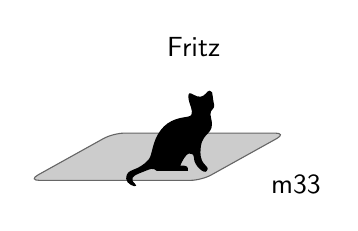
\begin{tikzpicture}[baseline=(fritz)]
  \begin{scope}[yshift=-1.2cm, xshift=-1.1cm, xslant=1.8]
    \filldraw [fill=black!20, draw=black!60, rounded corners] (0,0) rectangle (2.2,0.6);
  \end{scope}
  \Cat{black}
  \node [font=\sffamily] (fritz) at (1,0.5) {Fritz};
  \node [font=\sffamily] at (2.3,-1.25) {m33};
\end{tikzpicture}
\caption{Fritz the cat sits on a mat.}
\label{fig:cat}
\end{figure}


% Although record types will be represented in the above-given format, technically they involve functions \is{function} from individuals, not labels, to predicational types. 
% %
% That is, officially the \enquote{cat part} of the record type in (\ref{ex:fritz-situation}) has the following structure:
% %
% \ea \label{ex:official-notation}
% \begin{avm}
% \[
% x & : & \ttrtype{Ind} \\
% c1 & : & \<$\lambda v$:\ttrtype{Ind} . cat($v$), \q<x\q>\> 
% \]
% \end{avm}
% \z
% %
% The predicational type c1 from (\ref{ex:official-notation}) is a function from individuals onto cats, i.e.\ it is of the Montagovian type $\langle e,t \rangle$, where the object abstracted over is to be found at path x in the record type. 
% %
% This function is characterised by the set of ordered pairs $\{\langle v, \ttrtype{cat}(v) \rangle \mid v : \ttrtype{Ind} \}$ and thereby is linked to a set theoretical notion of extension.

Using type constructors, various types can be build out of basic and complex (dependent) types, such as set types and list types. 
%
In order to provide two (slightly simplified) examples of type constructors that will be useful later on, we just mention \emph{function types} \is{function type} and \emph{singleton types} \is{singleton type} here.

\ea Function type \label{ex:function}
\ea If $T_1$ and $T_2$ are types, then $(T_1 \rightarrow T_2)$ is a type, namely the type of functions that map $T_1$ to $T_2$.
\ex If a function $f$ is of type $(T_1 \rightarrow T_2)$ then $f$'s domain is $\{a \mid a : T_1\}$ and its range is included in $\{a \mid a : T_2\}$.
\z
\z 
%
The characterisation in (\ref{ex:function}) is that of a standard extensional notion of function. 
%
Given that TTR is an intensional semantic theory -- that is, two types are different even if their extension is the same -- other notions of function types could be developed.


\ea Singleton type
\ea If $T$ is a type and $a : T'$ (i.e.\ object $a$ is of type $T'$), then $T_a$ is a type.
\ex $b : T_a$ (i.e.\ object $b$ is of type $T_a$) iff $b : T$ and $b = a$.
\z
\z
%
That is, a singleton type is singleton since it is the type of specific object. 

Since types are semantic objects in their own right (types are not defined by or reduced to their extensions), not only an object $o$ of type $T$ can be the value of a label, but also  type $T$ itself.
%
One way of expressing this is in terms of 
\emph{manifest fields}. \is{manifest field}
%
A type-manifest field is notated in the following way: $l=T : T'$, specifying that $l$ is the type $T$.
%
Analogously, object-manifest fields can be expressed by restricting the value of a label to a certain object.


For more comprehensive and formal elaborations of TTR, see the references given at the beginning of this section, in particular \citet{Cooper:ms}.
\is{type theory|)} \is{Type Theory with Records|)} \is{type-theoretical semantics|)}



\is{dialogue gameboard|(} \is{KoS|(}
\section{Putting things together: \HPSGTTR and dialogue game boards}
\label{sec:hpsgttr-dialogue-game-boards}

Signs as construed within HPSG can be reconstructed as record types of a specific kind \citep{Cooper:2008}.
%
For instance, (\ref{ex:hpsgttr-sign}) shows the record type (the judgement colon indicates that we now talk about TTR objects) for a general \isi{sign} according to \citet{Pollard:Sag:1994} (where \ttrtype{PhonType}, \ttrtype{CategoryType} and \ttrtype{SemType} denote obvious types -- see the Appendix for a minimal HPSG fragment defined in terms of TTR).
%
\ea \label{ex:hpsgttr-sign}
\begin{avm}
\[
phon &:& \ttrtype{list}(\ttrtype{PhonType}) \\
synsem &:& 
    \[local &:&
        \[cat &:& \ttrtype{CategoryType} \\
        content &:& \ttrtype{SemType} \\
        context &:& \ttrtype{SemType}
        \]
    \]
\]
\end{avm}
\z

Signs are extended by an interface to \isi{circumstantial features} of the utterance situation in terms of the \textsc{dgb-params} \isfeat{dgb-params} attribute, which corresponds to the \textsc{c-inds} from Section~\ref{sec:c-inds-background}.
%
The attribute's name abbreviates \emph{dialogue gameboard parameters} \is{dialogue gameboard parameters}, since its values have to be instantiated (that is, witnessed) \is{witness} in the process of \isi{grounding}.
%
Thus, if the content of an NP $\alpha$ is part of \textsc{dgb-params}, then $\alpha$ gets a \isi{referential interpretation}.
%
However, NPs need not be used referentially; there are what \citet{Donellan:1966} calls \emph{attributive uses} \is{attributive use} as in \textit{The thief (whoever he is) stole my credit card}.
%
To this end, there is a \enquote{coercion} operation from \textsc{dgb-params} to \textsc{q-params} \isfeat{q-params} (\emph{quantificational parameters}) \is{quantificational parameters} involving an abstraction from individuals to $\alpha$'s descriptive condition (\citealt{Purver:Ginzburg:2004}; see the Appendix for the respective operation).


These \HPSGTTR signs figure as constituents within an architecture known as \emph{dialogue gameboard}, giving rise to a \isi{grammar-dialogue interface} within the dialogue theory \emph{KoS}
\citep{Ginzburg:1994,Ginzburg:1996,Ginzburg:2003,Ginzburg:2012}. 
%
A Dialogue Game Board (DGB) is an information-state based sheet for describing \isi{communicative interactions}.
%
The DGB from KoS tracks the interlocutors (\textit{spkr} and \textit{addr} fields), a record of the \isi{dialog history} (\textit{Moves}), dialogue moves that are in the process of \isi{grounding} (\textit{Pending}), the question(s) currently under discussion \is{question under discussion} (\textit{QUD}), the assumptions shared among the interlocutors (\textit{Facts}) and   the dialogue
participant's view of 
the \isi{visual situation} and attended entities (\textit{VisualSit}).
%
\is{proposition|(} \is{Austinian proposition|(} \is{locutionary proposition|(}
The TTR representation of a DGB following \citet{Ginzburg:2012} is given in (\ref{ex:dgb}), where \textit{LocProp} is the type of a \emph{locutionary proposition} (see (\ref{ex:locprop}) below) and \textit{poset} abbreviates \enquote{partially ordered set}.
%
\ea \label{ex:dgb}
\begin{avm}
\[
spkr & : & \ttrtype{Ind} \\
addr & : & \ttrtype{Ind} \\
utt-time & : & \ttrtype{Time} \\
c-utt & : &  addressing(spkr, addr, utt-time) \\
facts & : & set(\ttrtype{Prop}) \\
visualsit & : & \ttrtype{RecType} \\
pending & : & list(\ttrtype{LocProp}) \\
moves & : & list(\ttrtype{LocProp}) \\
qud & : & poset(Question) \\
\]
\end{avm}
\z


TTR, like many HPSG variants (e.g.\ \citealt{Pollard:Sag:1987} and \citealt{Pollard:Sag:1994}), employs a situation semantic domain \citep{Cooper:ms}.
%
This involves propositions being modelled in terms of types of situations, not in terms of sets of possible worlds.
%
Since TTR is a type theory, it offers at least two explications of proposition.
%
On the one hand, propositions can be identified with types \citep{Cooper:2005:b}.
%
On the other hand, propositions can be developed in an explicit Austinian \aimention{John Langshaw Austin} \citep{Austin:1950} way, where a proposition is individuated in terms of a \isi{situation} and \isi{situation type} \citep[\page 845]{Ginzburg:2011:a} -- this is the truth-making (and Austin's original) interpretation of \enquote{It takes two to make a truth}, since on Austin's conception a situation type can only be truth-evaluated against the situation it is about.
%
We follow the latter option here.
%
The type of propositions and the relation to a situation semantics \is{situation semantic} conception of \enquote{true} \citep{Barwise:Perry:1983} is given in (\ref{ex:propositions}):
%
\ea \label{ex:propositions}
\ea 
\begin{avm}
{\normalfont\ttrtype{Prop} $=_{\textit{def}}$} \[sit & : & \ttrtype{Record} \\ sit-type & : & \ttrtype{RecType}\]
\end{avm}
\ex 
\begin{avm}
{\normalfont A proposition $p =$}  \[sit & = & $s$ \\ sit-type & = & $T$\]\quad {\normalfont is true iff $s : T$}.
\end{avm}
\z
\z

A special kind of proposition, namely \emph{locutionary propositions} (\ttrtype{LocProp}) \citep[\page 172]{Ginzburg:2012}, can be defined as follows:
%
\ea \label{ex:locprop}
\begin{avm}
{\normalfont \ttrtype{LocProp} $=_{\textit{def}}$} \[sign & : & \ttrtype{Record} \\ sign-type & : & \ttrtype{RecType}\]
\end{avm}
\z
%
Locutionary propositions are sign objects utilized to explicate \isi{clarification potential} (see Section~\ref{sec:sub-sentential-meanings}) and \isi{grounding}. 
\is{proposition|(} \is{Austinian proposition|(} \is{locutionary proposition|(}

\is{interjections|(}
Given the dialogue-awareness of signs just sketched, a content for interjections such as \enquote{EHHH HEHH} which constitutes turn 3 from the exchange between Ann and Ray in (\ref{ex:ann-ray}) at the beginning of this chapter can be given.
%
Intuitively, Ann signals with these sounds that she heard Ray's question, which in turn is neither grounded nor clarified at this point of dialogue but is waiting for a response, what is called \emph{pending}. \is{pending}
%
This intuition can be made precise by means of the following lexical entry (which is closely related to the meaning of \textit{mmh} given by \citealt[\page 163]{Ginzburg:2012}):
%
\ea \label{ex:ehh-hehh}
\begin{avm}
\[
phon : \q< ehh hehh \q> \\
cat : \[head={\normalfont\ttrtype{interjection}} &:& \ttrtype{syncat}\] \\
dgb-params : \[spkr &:& \ttrtype{Ind} \\
              addr &:& \ttrtype{Ind} \\
              pending &:& \ttrtype{LocProp} \\
              c2 &:& address(spkr,addr,pending)
             \] \\
cont={\normalfont\ttrtype{Understand}}(spkr,addr,dgb-params.pending) : {\normalfont\ttrtype{IllocProp}}
\]
\end{avm}
\z

Knowing how  to use feedback signals \is{feedback} \is{feedback signal} such as the one in (\ref{ex:ehh-hehh}) can be claimed to be part of \isi{linguistic competence}.
%
It is difficult to imagine how to model this aspects of \isi{linguistic knowledge} if not by means of \emph{grammar in dialogue}.
\is{interjections|)}


\is{conversational rule|(}
Dialogue gameboard structures as defined in (\ref{ex:dgb}) as well as lexical entries for interjections such as (\ref{ex:ehh-hehh}) are still \emph{static}.
%
The mechanism that is responsible for the dynamics of dialogue and regiments the interactive evolution of DGBs is \emph{conversational rules}.
%
A conversational rule is a mapping between an input and an output information state, where the input DGB is constrained by a type labelled \emph{preconditions} (\textsc{pre}) \is{preconditions, conversational rule} and the output DGB is subject to \textsc{effects}.\is{effects, conversational rule}
%
That is, a conversational rule can be notated in the following form, where \ttrtype{DGBType} is the type of dialogue gameboards defined in (\ref{ex:dgb}).
%
\ea \label{ex:pre-effect}
\begin{avm}
\[
pre &:& \ttrtype{DGBType} \\
effects &:& \ttrtype{DGBType}
\]
\end{avm}
\z

Several basic conversational rules are defined in \citet[Chapter 4]{Ginzburg:2012} and some of them, namely those needed to analyse example (\ref{ex:Cambridge}) discussed above, are re-given below (with \enquote{Fact update/QUD-downdate} being simplified, however).
%
\textit{IllocProp} abbreviates \enquote{Illocutionary Proposition}, \textit{IllocRel} \enquote{Illocutionary Relation}, \textit{poset} \enquote{Partially Ordered Set}, \textit{AbSemObj} \enquote{Abstract Semantic Object} and \textit{QSPEC} \enquote{Question-under-Discussion-Specific}.
%
With regard to the partially ordered QUD set, we use \enquote{$\langle u, X\rangle$} to denote the upper bound $u$ for subset $X$.
%
For details, we have to refer the reader to \citet{Ginzburg:2012}; we believe the following list to convey at least a solid impression of how dialogue dynamics works in KoS, however.
%
\begin{itemize}
\item Free Speech:\par\medskip
\begin{avm}
\[
pre &:& \[qud=\q<\q> &:& poset(Question)\] \\
effects &:& TurnUnderspec \ttrmerge\ \[r : AbSemObj \\ R : IllocRel \\ LatestMove=R(spkr,addr,r) : IllocProp\] \\
\]
\end{avm}
\item QSPEC:\par\medskip
\begin{avm}
\[
pre &:& \[qud=\<q,Q\> &:& poset(Question)\] \\
effects &:& TurnUnderspec \ttrmerge\ \[r : AbSemObj \\ R : IllocRel \\ LatestMove=R(spkr,addr,r) : IllocProp \\ c1 : Qspecific(r,q)\] \\
\]
\end{avm}
\item Ask QUD-incrementation:\par\medskip
\begin{avm}
\[
pre &:& \[q &:& Question \\ LatestMove=Ask(spkr,addr,q) &:& IllocProp\] \\
effects &:& \[qud=\<q,pre.qud\> &:& poset(Question)\]
\]
\end{avm}
\item Assert QUD-incrementation:\par\medskip
\begin{avm}
\[
pre &:& \[p &:& Proposition \\ LatestMove=Assert(spkr,addr,p) &:& IllocProp\] \\
effects &:& \[qud=\<p?,pre.qud\> &:& poset(Question)\]
\]
\end{avm}
\item Accept:\par\medskip
\begin{avm}
\[
pre &:& \[spkr &:& Ind \\ addr &:& Ind \\ p &:& Prop \\ LatestMove=Assert(spkr,addr,p) &:& IllocProp \\ qud=\<p?,subqud\> &:& poset(Question)\] \\
effects &:& \[spkr=pre.addr &:& Ind \\ addr=pre.sprk &:& Ind \\ LatestMove=Accept(spkr,addr,p) &:& IllocProp\]
\]
\end{avm}
\item Fact update/QUD-downdate (simplified): 
\begin{itemize}
\item
\begin{avm}
\[
pre &:& \[q &:& Question \\ p &:& Prop \\ LatestMove=Accept(spkr,addr,p) &:& IllocProp \\ qud=\<q,subqud\> &:& poset(Question) \\ qbg &:& Qspecific(p,q) \] \\
effects &:& \[facts=pre.facts $\cup$ \{p\} &:& Set(Prop) \\ qud=pre.qud $\setminus$ \{q\}\] 
\]
\end{avm}
\item
\begin{avm}
\[
pre &:& \[p &:& Prop \\ LatestMove=Accept(spkr,addr,p) &:& IllocProp \\ qud=\<p?,subqud\> &:& poset(Question) \] \\
effects &:& \[facts=pre.facts $\cup$ \{p\} &:& Set(Prop) \\ qud=pre.qud $\setminus$ \{p?\}\] 
\]
\end{avm}
\end{itemize}
\end{itemize}


Having dialogue game boards and conversational rules at one's disposal, we can apply KoS' analytical tools to the dialogue example from (\ref{ex:Cambridge}) above.
%
We make the following simplifying assumptions: if the $n$th move is an assertion, we refer to the asserted proposition in terms of \enquote{p($n$)}. %
The corresponding question \textit{whether p($n$)} is notated \enquote{p?($n$)}.
%
If the $n$th move is a question, we refer to the question in terms of \enquote{q($n$)}.
%
Additionally, we assume that subsentential utterances project to Austinian propositions by resolving elliptical expressions in context in terms of their missing semantic constituents which are available as the contents of the maximal elements in QUD (that is, they are addressable via the path \textsc{qud.first.cont}; cf.  \citealt{Ginzburg:2012}). 

\tabulinesep=4pt
\begin{longtabu} to \linewidth {| @{}r | X[l,2.2] | X[l]@{} |}
\hline
\textbf{Turn} & \textbf{DGB dynamics} & \textbf{Utterance} / \textbf{Conversational rule(s)} \\
\hline 
init. 
&
\begin{avm}
\[
participants &=& \{A,B\} \\
Moves &=& \avmel \\
qud &=& \avmel \\
facts &=& cg0
\]
\end{avm}
&
---
\\
\hline
1. 
& 
\begin{avm}
\[
spkr &=& A \\
addr &=& B \\
Moves &=& \< Assert(A,B,p(1)) \> \\
qud &=& \< p?(1) \> \\
facts &=& cg0
\]
\end{avm}
& 
\enquote{I've been at university.}  \par\bigskip
Free Speech + Assert QUD-incrementation
\\
\hline
2.
&
\begin{avm}
\[
spkr &=& B \\
addr &=& A \\
Moves &=& \< Ask(B,A,q(2)), Assert(A,B,p(1)) \> \\
qud &=& \< q(2) \> \\
facts &=& cg0 $\cup$ \{p(1)\}
\]
\end{avm}
&
\enquote{Which university?} \par\bigskip
Accept + Ask QUD-incrementation
\\
\hline
3.
&
\begin{avm}
\[
spkr &=& A \\
addr &=& B \\
Moves &=& \< Assert(A,B,p(3)), \\ Ask(B,A,q(2)), Assert(A,B,p(1)) \> \\
qbg &=& About(p(3),q(2)) \\
qud &=& \< p?(3), q(2) \> \\
facts &=& cg0 $\cup$ \{p(1)\}
\]
\end{avm}
&
\enquote{Cambridge.} \par\bigskip
QSPEC (via \textit{About} relation) + Assert QUD-incrementation
\\
\hline
4.
&
\begin{avm}
\[
spkr &=& B \\
addr &=& A \\
Moves &=& \< Accept(B,A,p(3)), Assert(A,B,p(3)), \\ Ask(B,A,q(2)), Assert(A,B,p(1)) \> \\
qud &=& \avmel \\
facts &=& cg0 $\cup$ \{p(3), p(1)\}
\]
\end{avm}
&
\enquote{Cambridge, um.} \par\bigskip
Accept + Fact update/QUD-downdate
\\
\hline
5.
&
\begin{avm}
\[
spkr &=& B \\
addr &=& A \\
Moves &=& \< Ask(B,A,q(5)), \\ Accept(B,A,p(3)), Assert(A,B,p(3)), \\ Ask(B,A,q(2)), Assert(A,B,p(1)) \> \\
qud &=& \< q(5) \> \\
facts &=& cg0 $\cup$ \{p(3), p(1)\}
\]
\end{avm}
&
\enquote{what did you read?} \par\bigskip
Free Speech + Ask QUD-incrementation
\\
\hline
6.
&
\begin{avm}
\[
spkr &=& A \\
addr &=& B \\
Moves &=& \< Assert(A,B,p(6)), Ask(B,A,q(5)), \\ Accept(B,A,p(3)), Assert(A,B,p(3)), \\ Ask(B,A,q(2)), Assert(A,B,p(1)) \> \\
qbg &=& About(p(6),q(5)) \\
qud &=& \< p?(6), q(5) \> \\
facts &=& cg0 $\cup$ \{p(3), p(1)\}
\]
\end{avm}
&
\enquote{History and English.} \par\bigskip
QSPEC (via \textit{About} relation) + Assert QUD-incrementation
\\
\hline
7.
&
\begin{avm}
\[
spkr &=& B \\
addr &=& A \\
Moves &=& \< Accept(B,A,p(6)), \\ Assert(A,B,p(6)), Ask(B,A,q(5)), \\ Accept(B,A,p(3)), Assert(A,B,p(3)), \\ Ask(B,A,q(2)), Assert(A,B,p(1)) \> \\
qud &=& \avmel \\
facts &=& cg0 $\cup$ \{p(6), p(3), p(1)\}
\]
\end{avm}
&
\enquote{History and English.} \par\bigskip
Accept + Fact update/QUD-downdate
\\
\hline
\end{longtabu}


Note that the dialogical exchange leads to an increase of the common ground of the interlocutors A and B: after chatting, the common ground contains the propositions \textit{that A has been at university} (p(1)), \textit{that A has been at Cambridge University} (p(3)) and \textit{that A read History and English} (p(6)).
\is{conversational rule|)}
\is{dialogue gameboard|)} \is{KoS|)}


On these grounds, a lexical entry for \enquote{hello} can be spelled out.
%
\enquote{Hello} realises a greeting move (which is its content) and must be used discourse-initially (the \textsc{moves} list and the \textsc{qud} set have to be empty):
%
\ea
\begin{avm}
\[
phon : \q< hello \q> \\
cat : \[head=\textit{interjection} &:& \ttrtype{syncat}\] \\
dgb-params : \[spkr &:& \ttrtype{Ind} \\ 
               addr &:& \ttrtype{Ind} \\
               moves=\avmel &:& list(\ttrtype{IllocProp}) \\ 
               qud=\{\space\} &:& poset(\ttrtype{Question}) \] \\
cont=Greet(spkr,addr): \ttrtype{IllocProp}
\]
\end{avm}
\z 

Discourse-dynamically, \enquote{hello} puts a greeting move onto the \textsc{moves} list of the dialogue gameboard, thereby initiates an interaction and invites for a countergreeting (the requirement for countergreeting is exactly that a greeting move is the element of the otherwise empty list of dialogue moves) -- giving rise to an \emph{adjacency pair} \is{adjacency pair} as part of the \isi{local management system} for dialogues investigated in \isi{conversational analysis} \citep{Schegloff:Sacks:1973}.

The discourse particle \enquote{yes} can be used to answer a polar yes/no question. \is{polar question}
%
In this use, \enquote{yes} has a propositional content $p$ that asserts the propositional content of the polar question $p$?, which has to be the maximal element in \textsc{qud} \citep[Chapter 2, \page 231 \textit{et seq.}]{Ginzburg:2012}.
%
That is, \enquote{yes} affirmatively resolves a given polar question.
%
Polar questions, in turn, are 0-ary propositional abstracts \citep[\page 231]{Ginzburg:2012}, that is, the polar question $p$? corresponding to a proposition $p$ is a function mapping an empty record to $p$: $\lambda r : [] . p$.
%
Thus, applying $p$? to an empty record $[]$ returns $p$, which is exactly what \enquote{yes} does.
%
The affirmative particle (used to answer a yes/no question) is a propositional lexeme which applies a polar question which is maximal in \textsc{qud} to an empty record \citep[cf.][\page 232]{Ginzburg:2012}:
%
\ea
\begin{avm}
\[
phon : \q< yes \q> \\
cat : \[head=\textit{partcl} &:& \ttrtype{syncat}\] \\
dgb-params : \[qud=\[max &:& \ttrtype{PolQuestion} \\ rest &:& set(\ttrtype{Question})\] &:& poset(\ttrtype{Question}) \] \\
cont=dgb-params.qud.max( [\space] ): \ttrtype{Prop}
\]
\end{avm}
\z 
%
Due to its involvedness in \textsc{dgb-params.qud}, \enquote{yes} directly interacts with \isi{accept} and \isi{downdating}, as described above.
%
For more on this, see \citet{Ginzburg:2012}.



\section{Outlook}
\label{sec:outlook-dialogue}

Given a basic framework for formulating and analysing content in dialogue context, there are various directions to explore, including the following ones.

\begin{itemize}
    \item 
One of the main challenges of dialogue semantics is the integration of \emph{non-verbal communication} means, like gaze, gestures, body posture, timing and non-language  vocal sounds (e.g.\ laughter; \citealt{Ginzburg:Breitholz:Cooper:Hough:Tian:2015,Tian:Mazzocconi:Ginzburg:2016}).
%
Since \isi{non-verbal communication} means are informative, not only does a (dialogue) semantic representation have to be developed, but also the rules of their interaction with speech have to be formulated. 

\item Strictly speaking, dialogue is the interaction between \emph{two} interlocutors.
%
How can one scale up to \emph{multilogue}\is{multilogue}, where the number of participants is at least three \citep{Ginzburg:Fernandez:2005}?
%
Given the increased number of participants,  problems that emerge include  \emph{grounding by proxy}, \is{grounding} where a representative represents the dialogue gameboard of a group \citep{Eshghi:Healey:2016} and of course \emph{turn taking}.

\item People do not process natural language input sentence-wise.
%
Rather, processing begins with the initial sound and proceeds word for word or even on smaller units like affixes and phonemes -- that is, processing is incremental \is{incremental} \is{incremental processing} (e.g.\ \citealt{Sedivy:Tanenhaus:Chambers:Carlson:1999}; see also \crossrefchapteralt{processing}). This is a key ingredient in the efficient (relatively gap-free and interruption-less) managing of turn taking.
%
One direction of dialogue theories therefore is to bring psycholinguistics and formal semantics closer together by devising incremental grammar and dialogue gameboard models \citep{Hough:Kennington:Schlangen:Ginzburg:2015,Demberg:Keller:Koller:2013,Poesio:Rieser:2011}.

\end{itemize}


Finally, we want to mention two other dialogue-theoretic frameworks that have been worked out to a substantial degree, namely \isi{PTT} \citep{Traum:1994,Poesio:1995,Poesio:Traum:1997,Poesio:Rieser:2010}, and \emph{Segmented Discourse Representation Theory} \is{Segmented Discourse Representation Theory} (SDRT) \citep{Asher:1993,Asher:Lascarides:2003,Asher:Lascarides:2013,Hunter:Asher:2015}.
%
The phenomena and outlook directions discussed in this chapter apply to all theories of dialogue semantics, of course. 




\is{HPSG-TTR|(}
%\appendix
\section*{Appendix: An \HPSGTTR fragment}

The appendix provides a fragment of \HPSGTTR.
%
The grammar framework used is oriented at a \textit{Head-driven Phrase Structure Grammar} variant \citep{Sag:Wasow:Bender:2003}, namely its TTR implementation \citep{Cooper:2008}.
%
We use HPSG because its  architecture satisfies the property of \emph{incremental correspondence} \citep{Johnson:Lappin:1999} -- utterance representations encode phonological, syntactic, semantic and contextual information \emph{fractally}.
%
 This is crucial {\it inter alia} for any treatment of clarification interaction (cf. Section~\ref{sec:sub-sentential-meanings}). 
%
We use HPSG\textsubscript{TTR} because the type-theoretical version allows us to directly incorporate semantic objects (cf. Section~\ref{sec:semantic-objects}).


TTR has a counterpart to unification, namely the \emph{merge} construction.
%
\ea
\ea If $R_1$ and $R_2$ are record types, then $R_1 \ttrmerge R_2$ is a record type and is called the \emph{merge} of $R_1$ and $R_2$.
\ex Since merge types are complicated to define \citep[but see][]{Cooper:2012}, we follow the strategy of \citet{Cooper:2017:a} and illustrate the working of merges by means of some examples:
\begin{enumerate}[label=(\roman*), leftmargin=6.5em]
\item 
\begin{avm}
\[a &:& $T$ \\ b &:& $R$\]
\quad\ttrmerge\space\space
\[c &:& $S$\]
\quad = \space
\[a &:& $T$ \\ b &:& $R$ \\ c &:& $S$\]
\end{avm}
%%
\item 
\begin{avm}
\[a &:& $T$ \]
\quad\ttrmerge\space\space
\[a &:& $R$ \]
\quad = \space
\[a &:& $T$ \ttrmerge\ $R$\]
\end{avm}
\end{enumerate}
\z
\z


Structure sharing is indicated by a \enquote{tag type} notation.
%
Tag types are defined in terms of manifest fields.\footnote{\textit{NB:} technically, tag types apply singleton types to record types, instead of to objects, thereby making use of a revision of the notion of singleton types introduced by \citet[4, footnote~3]{Cooper:2013}.}
%
The notational convention is exemplified in (\ref{ex:tag-notation}) by means of head-specifier agreement, where the tag type from (\ref{ex:tag-notation}a) abbreviates the structure in (\ref{ex:tag-notation}b):
%
\ea \label{ex:tag-notation}
\ea
\begin{avm}
\[
cat &:& \[head &:& \[agr$_{\@{1}}$ &:& \ttrtype{Agr}\] \\
          spr &:& \<[cat &:& \[head &:& \[agr=\@{1} &:& \ttrtype{Agr}\]\]\>
        \]
\]
\end{avm}
\ex 
\begin{avm}
\[
cat &:& \[head &:& \[agr &:& \ttrtype{Agr}\] \\
          spr &:& \<[cat &:& \[head &:& \[agr=/cat.head.agr &:& \ttrtype{Agr}\]\]\>
        \]
\]
\end{avm}
\z
\z 
%
The tag type notation alludes to the box notation common in HPSG work.


\ttrtype{Agr} is defined as usual:
%
\ea
\ttrtype{Agr} $\coloneqq$
\begin{avm}
\[num &:& \ttrtype{Num} \\
pers &:& \ttrtype{Per} \\
gen &:& \ttrtype{Gen}
\]
\end{avm}
\z 

% The grammar framework makes use of some grammar-specific types, which are enumerated (partly employing obvious abbreviations) in the following:
% %
% \begin{itemize}
% \item Parts of speech: \ttrtype{noun}, \ttrtype{verb}, \ttrtype{prep} \ldots of type \ttrtype{PoS};
% %%
% \item Type of constituent: \ttrtype{lexeme}, \ttrtype{word}, \ttrtype{phrase};
% %%
% \item Number: \ttrtype{sg}, \ttrtype{pl} of type \ttrtype{Num};
% %%
% \item Person: \ttrtype{1st}, \ttrtype{2nd}, \ttrtype{3rd} of type \ttrtype{Pers};
% %%
% \item Gender: \ttrtype{fem}, \ttrtype{masc}, \ttrtype{neut} of type \ttrtype{Gend};
% %%
% \item Case: \ttrtype{nom}, \ttrtype{acc}, \ttrtype{gen}, \ttrtype{dat} of type \ttrtype{Case};
% %%
% \item A type \ttrtype{Phoneme} which captures phonetic representations (which are simplified in terms of orthographic transcriptions);
% %%
% \item Semantic objects: \ttrtype{Ind}, \ttrtype{Quant}, \ttrtype{Prop}, \ttrtype{Set}(\ttrtype{Ind}), \ldots\ of type \ttrtype{SemObj} (see  \textcite{Ginzburg:2012} for more on \ttrtype{SemObj});
% %%
% \item The type \ttrtype{SynCat} takes care of syntactic information and includes fixed path names like \enquote{head}, \enquote{spr} (specifier), \enquote{comps} (complements);
% %%
% \end{itemize}


A basic \emph{sign} is a pairing of phonetic, syntactic and semantic information and follows the geometry in (\ref{ex:sign}): 
%
\ea \label{ex:sign}
\ttrtype{sign} $\coloneqq$ 
\begin{avm}
\[
phon &:& \ttrtype{Phoneme} \\
cat &:& \ttrtype{SynCat} \\
dgb-params &:& \ttrtype{RecType} \\
cont &:& \ttrtype{SemObj} \\
\]
\end{avm}
\z

Signs employ \textsc{dgb-params}, which host referential meanings that are witnessed among interlocutors. 
%
Quantificational abstraction is achieved by coercing parts of \textsc{dgb-params} to \textsc{q-params}:
%
\ea
If \textsc{dgb-params} : $R_2$ and for two record types $R_0$ and $R_1$ lacking any mutual dependencies\footnote{None of the labels occurring in $R_0$ occur in $R_1$ and vice versa.}
$R_2 = R_0 \wedge_{merge} R_1$,
 % $R_0 \sqsubseteq R_1$
then $R_0$ can be moved to \textsc{q-params}, resulting in the following structure: \par\medskip 
 % \commentrhc{You should explain what you mean by $\setminus$. We would need an example to make sure this is working. }
 
\begin{avm}
\[
dgb-params &:& $R_1$\\
%\setminus R_0$ \\
cont &=& \[q-params &:& $R_0$\]
\]
\end{avm}
\z



A word is a sign with constituent type (\textsc{cxtype}) \ttrtype{word}.
%
Using the merge operation, the word extension on signs can represented compactly as in (\ref{ex:word}a), which expands to the structure given in (\ref{ex:word}b):
%

\ea \label{ex:word}
\ea \ttrtype{word} $\coloneqq$ \ttrtype{sign} \ttrmerge\ \begin{avm}
\[cxtype &:& \ttrtype{word}\]
\end{avm} : \ttrtype{RecType}
\ex 
\begin{avm}
\[
cxtype &:& \ttrtype{word} \\
phon &:& \ttrtype{Phoneme} \\
cat &:& \ttrtype{SynCat} \\
dgb-params &:& \ttrtype{RecType} \\
cont &:& \ttrtype{SemObj} 
\]
\end{avm}
\z
\z

Words -- that is, cxtype \ttrtype{word} -- are usually the result of lexical rules, whose input are lexemes.
%
Lexemes differ from words in their constituent type:
%
\ea
\ttrtype{lexeme} $\coloneqq$ \ttrtype{sign} \ttrmerge\ \begin{avm}
\[cxtype &:& \ttrtype{lexeme}\]
\end{avm} : \ttrtype{RecType}
\z

A phrasal sign can be seen as a word with daughters:
%
\ea 
\ea \ttrtype{phrase} $\coloneqq$ \ttrtype{sign} \ttrmerge\ \begin{avm}
\[cxtype &:& \ttrtype{phrase} \\
dtrs &:& \[nhd-dtrs &:& \ttrtype{List}(\ttrtype{Sign})\]\]
\end{avm} : \ttrtype{RecType}
\ex 
\begin{avm}
\[
cxtype &:& \ttrtype{phrase} \\
phon &:& \ttrtype{List}(\ttrtype{Phoneme}) \\
cat &:& \ttrtype{SynCat} \\
dgb-params &:& \ttrtype{RecType} \\
cont &:& \ttrtype{SemObj} \\
dtrs &:& \[% hd-dtr &:& \ttrtype{Sign} \\
           nhd-dtrs &:& \ttrtype{List}(\ttrtype{Sign})
         \]
\]
\end{avm}
\z
\z

A headed phrase is a phrase with a prominent daughter, i.e.\ the head daughter:
%
\ea 
\ea \ttrtype{hd-phrase} $\coloneqq$ \ttrtype{phrase} \ttrmerge\ 
\begin{avm}
\[dtrs &:& \[hd-dtr &:& \ttrtype{Sign}\]\]
\end{avm} : \ttrtype{RecType}
\ex 
\begin{avm}
\[
cxtype &:& \ttrtype{phrase} \\
phon &:& \ttrtype{List}(\ttrtype{Phoneme}) \\
cat &:& \ttrtype{SynCat} \\
dgb-params &:& \ttrtype{RecType} \\
cont &:& \ttrtype{SemObj} \\
dtrs &:& \[hd-dtr &:& \ttrtype{Sign} \\
           nhd-dtrs &:& \ttrtype{List}(\ttrtype{Sign})
         \]
\]
\end{avm}
\z
\z

The head daughter is special since it (as a default, at least) determines the syntactic properties of the mother construction. 
%
This aspect of headedness is captured in terms of the \emph{head-feature principle} (HFP), which can be implemented by means of tag types as follows:
%
\ea \label{ex:HFP}
HFP $\coloneqq$
\begin{avm}
\[
cxtype &:& \ttrtype{phrase} \\
cat &:& \[head$_{\@{2}}$ &:& \ttrtype{PoS}\] \\
dtrs &:& \[hd-dtr &:& \[cat &:& \[head=\@{2} &:& \ttrtype{PoS}\]\] \\
         \]
\]
\end{avm}
\z

The fact that the daughters' locutions combine to the mother's utterance is captured in terms of a \enquote{phon principle}  (we use a slash notation in order to indicate paths starting at the outermost level of a feature structure):
%
\ea 
PHON $\coloneqq$ \label{ex:phon-principle}
\begin{avm}
\[
cxtype &:& \ttrtype{phrase} \\
phon &:& \ttrtype{List}(/dtrs.hd.dtr/phon, /dtrs.nhd.dtrs/pos1.phon,  \\ && \ldots, /dtrs.nhd.dtrs/pos$n$.phon) 
% dtrs &:& \[hd-dtr &:& \ttrtype{Sign} \\
%           nhd-dtrs &:& \ttrtype{List}(\ttrtype{Sign})
%         \]
\]
\end{avm}
\z 

Since  semantic composition rests on predication rather than unification, there is no analog to the semantic compositionality principle of \citet{Sag:Wasow:Bender:2003} in our account.
%
There is, however, something akin to semantic inheritance: we need to keep track of the contextual and quantificational paramaters contributed by the daughters of a phrase. 
%
This is achieved in terms of a \emph{dgb-params principle} (\ttrtype{DGBPP}) in (\ref{ex:dgbpp}) which unifies the daughters' \textsc{dgb-params} into the mother's \textsc{dgb-params}  (see \citealt[126 \textit{et seq.}]{Ginzburg:2012}  for a similar principle): 
%
\ea \label{ex:dgbpp}
DGBPP $\coloneqq$ \label{ex:QPP} \par\medskip
\oneline{%
\begin{avm}
\[
cxtype &:& \ttrtype{phrase} \\
dgb-params &:& \[/dtrs.hd-dtr.dgb-params\ \ttrmerge\ /dtrs.nhd-dtrs.pos1.dgb-params\ \ttrmerge \\ \ldots \ttrmerge\ /dtrs.nhd-dtrs.pos$n$.dgb-params
             \] \\
dtrs &:& \[hd-dtr &:& \[q-params &:& \ttrtype{RecType}\] \\
           nhd-dtrs &:& \<pos1 &:& \[q-params &:& \ttrtype{RecType}\],  
                         \ldots, 
                         pos$n$ &:& \[q-params &:& \ttrtype{RecType}\]
                        \>
         \]
\]
\end{avm}
}
\z

A headed phrase is well-formed when it is a headed phrase and it obeys the head feature principle, the phon principle and the dgb-params principle, which is expressed by extending \ttrtype{hd-phrase} by the following constraint:
%
\ea \label{ex:hd-phrase}
\ttrtype{hd-phrase} $\coloneqq$ 
\ttrtype{hd-phrase} \ttrmerge\ {HFP} \ttrmerge\  {PHON} \ttrmerge\ {DGBPP}
\z


Using this set-up, lexical entries, lexical rules and syntactic constructions can be formulated straightforwardly. 
\is{HPSG-TTR|)}


%}% end avmoptions
 
% \section*{Abbreviations}
\section*{Acknowledgements}


The work on this chapter by Lücking is partially supported by a public grant overseen by the French National Research Agency (ANR) as part of the program ``Investissements d'Avenir'' (reference: ANR-10-LABX-0083). It contributes to the IdEx Université de Paris -- ANR-18-IDEX-0001. Cooper's work was supported by the projects InCReD (Incremental Reasoning in Dialogue), VR project 2016-01162 and DRiPS (Dialogical Reasoning in Patients with Schizophrenia), Riksbankens jubileumsfond, P16-0805:1 and a grant from the Swedish Research Council (VR project 2014-39) for the establishment of the Centre for Linguistic Theory and Studies in Probability (CLASP) at the University of Gothenburg. The authors want to thank several anonymous reviewers for their comments. We thank in particular Bob Borsley, Stefan Müller and Frank Richter for detailed discussions and suggestions on earlier drafts of this chapter. Furthermore, we are grateful to Elizabeth Pankratz for her attentive remarks and for proofreading. 

}% end avmoptions


{\sloppy
\printbibliography[heading=subbibliography,notkeyword=this]
}


\end{document}
